\chapter{RoomZoner: Room-Level Zoning}
\label{ch:cs2}

% Overview

Case study 1 (Chapter~\ref{ch:cs1}) was a preliminary analysis into the
feasibility of retrofitting a centralized HVAC system to enable two distinct
zones: a day zone and a night zone. Case study 2 involves the implementation of
{\em RoomZoner}: a room-level HVAC zoning system where each room is individually
conditioned based on its occupancy and temperature. RoomZoner dynamically change
zones in response to occupancy and temperature changes within rooms. An
occupancy assessment technique that relies on simple motion sensors is used to
decide when rooms become occupied and vacant and a simple thermal model of the
house to predict the effect of control decisions. Using this information
RoomZoner responds to changes in occupancy by redirecting conditioned
air through the house. This approach is based on the concept of Micro-zoning
which allows an HVAC schedule for individual rooms to be
customized~\cite{Airgonomix2008}. Rose and Dozier observed that micro-zoned
systems report energy savings of up to 43\% compared to conventional HVAC
systems with larger zones~\cite{rose1997epa}. The main contribution of RoomZoner
is that each zone is controlled based on occupancy.

RoomZoner involves a novel occupancy assessment technique and a zone control
algorithm that ensures the safety of HVAC hardware while attempting to minimize
energy wastage without compromising occupant comfort. The occupancy assessment
technique enables simple motion sensors, like those found in most residential
security systems, to be used to accurately infer rooms that are occupied and
distinguish them from rooms that being used only temporarily such as those that
serve as hallways between other rooms. The zone controller attempts to maintain
occupied rooms at a comfortable setpoint and ensure unoccupied rooms can be
conditioned to the setpoint within a short time of occupancy. It also ensures
the safety of the HVAC hardware by ensuring the system is not being turned on
and off too frequently or too much pressure is being built up within the
ducts due to the dampers to too many rooms being closed. A study carried out
over two months indicates that room-level zoning, with RoomZoner, consumes 14\%
less energy than whole house conditioning. 

\section{Background and Related Work}
\label{sec:cs2relatedWork}

Several previous studies have explored the possibility of room-level zoning, but
the conclusions of these studies have been mixed and
inconclusive~\cite{walker2003register,watts2007application,Systems2003}. RoomZoner
addresses this shortcoming with a long-term deployment in a residence which is
instrumented to enable occupancy to be monitored and the HVAC system controlled
in response to the occupancy. RoomZoner responds to changes in occupancy using
an occupancy assessment technique that relies on simple occupancy sensors. Many
different techniques for tracking occupants through a home, identifying them,
and understanding what activities they are doing have been proposed. Until
recently, however, existing technologies have all been too expensive or
intrusive for use in energy conservation applications. For example, some systems
require the user to wear a tag~\cite{smith2005rfid}, or to actively trigger a
biometric sensor such as a thumbprint or retina scanner. Other systems require
cameras to be installed in the home~\cite{nait4activity} and identify people,
locations, and activities using gait analysis, form matching, or face
recognition. However, cameras are often perceived to be invasive to personal
privacy. Other systems require structural changes to the home such as the
installation of smart floors, which incur a high initial cost and effort that
cannot be justified by applications in energy conservation. Finally, some
systems detect user activities by requiring a large set of training data that
must be laboriously collected for weeks or even months after the original sensor
deployment~\cite{wilson2005simultaneous}.

Unlike other smart home applications that rely on fine-grained activity
recognition, RoomZoner does not require cameras or wearable tags that may be
considered intrusive to the user; in contrast to other smart home applications
such as medical monitoring and security, this domain can tolerate a small loss
in accuracy in favor of cost and ease of use. Therefore, RoomZoner utilizes
commercial off the shelf (COTS) motion sensors, which cost approximately \$5
each. These sensors are wireless and can be installed in minutes using
double-sided tape. Evaluations of a similar system in eight homes have been able
to identify occupancy and sleep activities with over 90\%
accuracy~\cite{srinivasan2008protecting, srinivasan2010using}. We evaluate the
raw sensor readings with a novel occupancy assessment approach to distinguish
rooms that are actively being used from those that are transiently occupied as
residents pass through them.

RoomZoner uses a reactive thermostatic control scheme. Reactive control is one
of the three common types of HVAC thermostatic control mechanisms, the other two
being manual and programmable thermostats~\cite{thermostatHistory}. While
thermostats differ in the way they operate depending on what category they fall
into, they all attempt to trade off energy savings for occupant comfort.

Manual thermostats maintain the temperature of the house, or zone, it is
monitoring at a temperature to which it is currently configured, the
setpoint. With conscientious users, who setback the temperature when they leave
the house and go to bed and return the temperature to a comfortable level only
when they are active around the house, manual thermostats can be the most energy
efficient type of thermostat. Yet, they place a tremendous burden on the user to
constantly set the temperature based on his/her current activity. Also, the fact
that manual thermostats only start heating or cooling a house after the
residents return, or wake up, results in the resident having to endure periods
of discomfort while the house is warming up or cooling down. These reasons
result in over 65\% of residents with manual thermostats not switching to a
setback temperature when they vacate their houses~\cite{manualSetback}.

%------------------------------------------------------------------------------
% Figure 1
\begin{figure*}[t]
\centering{
  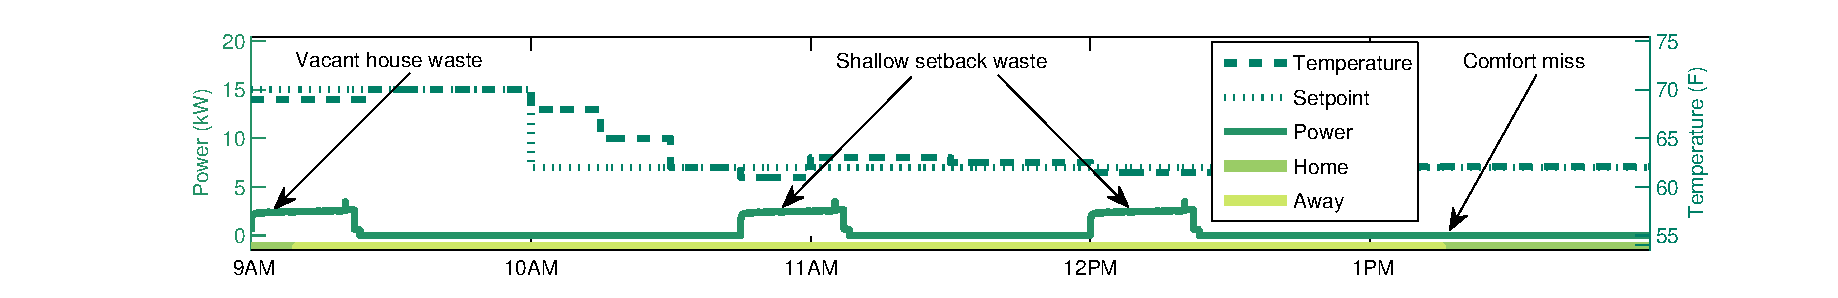
\includegraphics[width=0.8\columnwidth]{fig/scheduled}
} \caption[Drawbacks of Programmable Thermostats]{Programmable thermostats cause substantial energy waste and
  discomfort.} 
\label{fig:overviewScheduled}
\end{figure*}
%------------------------------------------------------------------------------
  
Programmable thermostats operate on a pre-defined {\em setback schedule}: the
house is conditioned to a setpoint temperature when the occupants are typically
active, and floats to a more energy efficient setback temperature when the
occupants are typically away or asleep. This approach wastes energy in several
ways, as illustrated by the composite of data traces in
Figure~\ref{fig:overviewScheduled} that were collected from a home using a
programmable thermostat. First, the occupants leave the home shortly after 9am,
but the system wastes energy because it is scheduled to continue heating the
home until 10am (left side). Second, the setback temperature is well above
safety limit for a home, causing energy consumption even while the house is
vacant (center). This type of {\em shallow setback} is typically used as a
safety precaution, in case the building actually is occupied at that
time. Third, the occupants become uncomfortable when they return shortly after 1
pm because the system is not scheduled to heat the house until much later. This
causes people to reduce their use of setback schedules, or stop using them
altogether. Over 50\% of households that have programmable thermostats are
reported to not use setback periods at night or during the
day~\cite{sumfindings}. In contrast, households with the simpler dial-type
thermostats can easily adjust temperature settings before going to sleep or
leaving the house, and as a result actually save more energy on average than
households with programmable thermostats\cite{sumfindings, sachs04}.

Reactive thermostats use motion sensors, door sensors, or card key access
systems to turn the HVAC equipment on and off based on occupancy. However,
preliminary studies of such systems in residential buildings have demonstrated
less energy savings than programmable thermostat and even increased energy usage
by up to 10\%~\cite{gao2009self}. Some commercial buildings are beginning to use
occupancy sensors to create a tighter link between occupancy and HVAC control
with reactive thermostats that use motion, window, and/or door sensors to turn
the HVAC system on or off after detecting that the occupants have left or
returned to a space. For example, the Telkonet SmartEnergy~\cite{telkonet}
control system allows the user to define a maximum recovery time parameter,
which is set by the user. When the space is unoccupied, the system maintains a
setback temperature from which it can return to the setpoint within the
specified recovery time, once the occupants return. The system estimates the
response time based on building and system parameters as well as current weather
conditions. Other similar commercial systems include the
Verdant~\cite{prothermostats}, Viconics~\cite{vt7000}, and PECO~\cite{peco}
systems. While reactive thermostats are a step in the right direction, they are
almost always applied to hotel rooms because they rely on the simplicity of
hotel rooms and the keyed entrance to identify occupants; more complex spaces
with multiple rooms, entrances, and occupants require more advanced sensing
technology, such as the techniques discussed in this proposal.

\label{sec:occupantOrientedHVACControl}
%------------------------------------------------------------------------------
% Figure 1
\begin{figure*}[t]
\centering{
  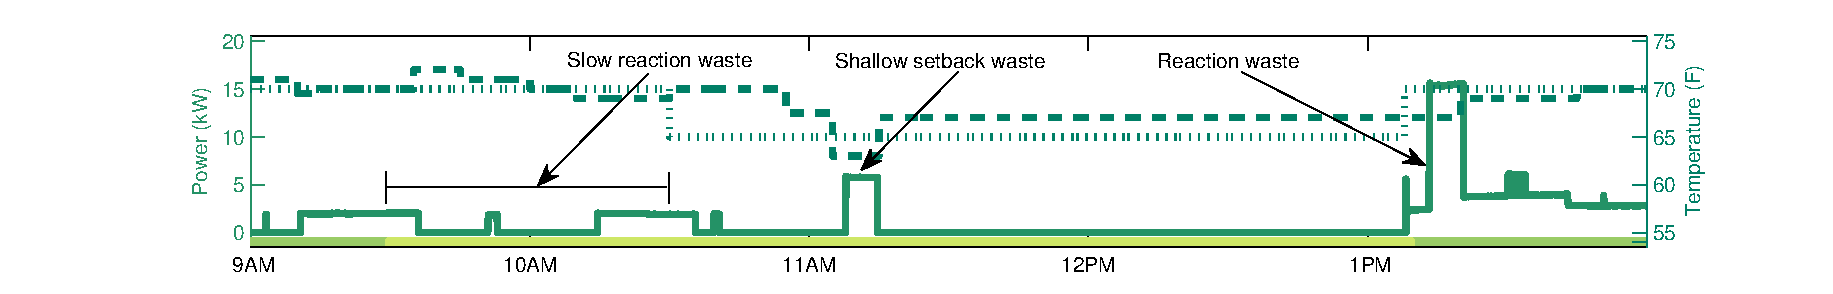
\includegraphics[width=0.8\columnwidth]{fig/reactive}
} \caption[Drawbacks of Occupant-oriented Thermostats]{Occupant-oriented thermostats have three sources of energy waste.} 
\label{fig:overviewReactive}
\end{figure*}
%------------------------------------------------------------------------------

Thermostatic control wastes energy due to occupancy patterns varying from the
pre-defined schedule, and the system having to maintain a setback temperature
close to the setpoint temperature so as to minimize discomfort if the occupants
become active unexpectedly (Figure~\ref{fig:overviewReactive}). In order to
remove the burden of having the program a thermostat based on occupancy
patterns, the {\em self-programming thermostat} which automatically chooses the
optimal setback schedule was proposed~\cite{gao2009self}. This system does not
fully solve the problems because occupancy patterns change every day, and so
{\em any} static schedule must either waste energy or sacrifice occupant
comfort.

{\em Smart Thermostat} was implemented as an extension to the self-programming
thermostat. It incorporated dynamic actuation in order to minimize the energy
wastage and loss of comfort due to variations in occupancy
patterns~\cite{Lu2010}. A Hidden Markov Model (HMM) was trained with data
collected from eight homes over a period of two weeks using leave-one-out
cross-validation. This model was used to predict occupancy and control a
mult-stage HVAC system. While this approach goes a long way in minimizing the
energy consumed by not conditioning an unoccupied house, there is still a lot of
savings to be had by not conditioning unoccupied spaces of an occupied house.

Gupta et al.~\cite{gupta2009adding} add GPS-control to traditional thermostats
by using information from location aware mobile phones to augment thermostats
with the ability to control HVAC systems using travel time. By estimating how
long it takes for the residents to return to an unoccupied home, the thermostat
can be placed in a ``just-in-time'' travel-to-home-time mode so that it starts
conditioning the house in time for the residents' arrival, thus staying in a
lower-power setback mode for longer. Through simulations, the authors
demonstrate energy savings of up-to 7\% in certain households. While this system
is one solution to the problem of efficiently using programmable thermostats, it
generally results in lower savings than programmable or manual thermostats and
does not provide any energy savings in heating or cooling occupied houses.

Mozer et al. present the {\em Neurothermostat} which uses daily occupancy
schedules and a neural network trained on five months of occupancy data in order
to control an HVAC system~\cite{mozer1997neurothermostat}. The authors
demonstrate that the Neurothermostat results in a lower unified cost, defined as
a combination of energy usage and occupant discomfort. 

Previous researchers have also investigated using multiple temperature sensors
in a building with a single thermostat~\cite{lin2002multi}. This work, done in
simulation, demonstrated an increase in user comfort by using targeted comfort
control strategies. Others retrofitted a house in Danville, CA with wirelessly
controllable registers and demonstrated that energy savings is possible by
directed air into localized zones~\cite{watts2007application}. This work did not
use occupant information to control the HVAC system.

% wireless systems 

Commercial buildings often use zoning systems that divide a single floor into
multiple rooms.  This is especially common in hotels, banquet halls, and office
buildings.  For example, the discharge-air-regulation technique (DART) uses
temperature sensors to control the HVAC fan
speed~\cite{federspiel2006wireless}. Other systems include the Millennial
Net~\cite{Net2009} and Siemens APOGEE~\cite{Inc.2010}.  Just like the
residential zoning systems, these solutions are expensive and are much easier to
add to a new installation.  Similarly, micro-environment systems (also called
task-ambient conditioning) allow a worker in an office building to have
fine-grained control over the ambient conditions around his or her working
space, typically a desk. Several systems, including Personal Environments from
Johnson Controls~\cite{Controls2010} and Habistat from Interface Architectural
Resources, are currently commercially available. The individually controlled
spaces are not insulated from each other and operate within a single thermal
zone. These systems are designed for occupant comfort over energy efficiency.
The systems can produce some energy savings by not conditioning desks that are
not occupied, and several studies have shown substantial savings of
micro-environment systems~\cite{Airgonomix2008,rose1997epa,llc2002energy}.
However, the cost of these systems is between \$20,000 and \$100,000 per desk,
which is too large to produce a positive return on investment.  Furthermore,
this approach is designed for offices and would be difficult to transfer to
homes, where usable space can be more difficult to instrument than a desk or
cubicle.

Finally, there have been patents filed for occupancy-based zoning of HVAC
systems using security systems~\cite{cohen2008hvac} or motion
sensors~\cite{simmons2002energy} to detect occupancy. While these systems
attempt to solve the problem addressed by RoomZoner, the effectiveness
of their approach is not evaluated. Also, these systems fail to address hardware
safety concerns that arise with implementing room-level zoning using a
centralized HVAC system. RoomZoner is cognizant of the short-cycling and
back-pressure that could reduce the lifespan of HVAC hardware and attempts to
minimize the potential damage to hardware.

\section{Occupancy Assessment}
\label{sec:occupancyAssessment}

%% - Detect when rooms used

%% - Anecdote example of ``IDEAL''
%%  - Person starts using -> ``Occupied''
%%  - Stops               -> ``Unoccupied'' 

RoomZoner aims to minimize the energy wasted when rooms that are unoccupied are
conditioned. Therefore, the goal of occupancy assessment is to detect when rooms
are used. In an ideal scenario, at night when two residents are asleep, only the
bedroom would be detected as being occupied. When one of the residents wakes up
in the morning and goes into the bathroom, the bathroom would be detected as
being occupied in addition to the bedroom. When the resident leaves the bathroom
and enters the kitchen, the bathroom would be detected as being unoccupied and
the kitchen would be detected as being occupied. Thus, as soon as a room starts
being used it should be detected as occupied and as soon as it stops being used
it should be detected as unoccupied.

%% - Find room usage with time constants commensurate with equipment operation

Such room usage detection is ideal for the control of systems such as lights
or faucets where the required service is provided almost immediately when it is
activated and can be deactivated instantly when the service is not needed, with
no repercussions. An HVAC system, in contrast, takes time to heat or cool a
space and turn off, and therefore cannot react to occupants entering and leaving rooms
without sacrificing comfort and efficiency. Therefore, assessing room occupancy
goes beyond merely detecting when a room starts being used and stops being
used. The occupancy assessment algorithm for RoomZoner has to find room usage
time constants commensurate with equipment operation periods. For instance, if
the HVAC system takes 15 minutes to heat the bathroom by one degree and the
resident enters and leaves the bathroom within a minute, detecting this
occupancy and reacting to it would waste energy while providing no benefit in
terms of comfort. Therefore, in assessing room occupancy, the system has to take
into consideration the HVAC equipment operation parameters.

%% - No short cycling -> Either damage -or- waste -or- discomfort | balance

Another issue that has to be considered when assessing occupancy is the short
cycling of HVAC equipment. Short cycling is the transition of the HVAC system
from an operating stage to a lower stage before the manufacturer recommended
minimum time. For instance, changing from stage 2 heat to stage 1 heat or
turning off from stage 1 cool before the minimum operating time for that
stage. Short cycling the HVAC system can cause equipment damage due to increased
wear and tear as a result of frequent equipment cycling and not allowing the
pressure within the system to equalize between cycles. 

In addition to potentially damaging hardware, short cycling could also waste
energy and subject the residents to discomfort. For instance, if a resident
spends most of his/her day in the living room but goes to the kitchen
periodically to get water or a snack, if the system did not consider short
cycling, the HVAC would turn off whenever the resident left the kitchen assuming
the living room was at the setpoint and the kitchen drifts away from the
setpoint due to being used infrequently. This turning on and off of the
equipment would waste energy while not providing any benefit to the
resident. Also, by allowing the kitchen to drift away from the setpoint, the
system would expend a large amount of energy in conditioning it when it is
used for a long period of time, such as when the resident is preparing a
meal. Similarly, short cycling the system would mean a room that is used
infrequently in conjunction with another room would never reach the setpoint
since the system turns off whenever the room stops being used. Thus, every time
the occupant enters the room s/he would be in discomfort. If occupancy
assessment only considered if a room was used or not in order to define it as
occupied or unoccupied, and actuated the HVAC system in response to this
information, short cycling would be inevitable. Thus, a more sophisticated
approach to occupancy assessment is needed as will be described below.

\subsection{Challenges}
\label{sec:occupancyAssessmentChallenges}

The challenges in assessing occupancy in most houses arise from room usage
durations not matching equipment operation periods and errors inherent in
sensing hardware. The mismatch in room usage durations and equipment operation
periods can manifest itself in {\em passageway rooms}, {\em multi-room usage},
and {\em short-term room usage}. Inadequacies of hardware usually manifest
themselves as false positives or negatives. In this section these four
challenges to occupancy assessment are described.

%% - Passageway rooms
\subsubsection{Passageway Rooms}
Passageway rooms are rooms, such as hallways, which connect two or more other
rooms. These could be central rooms in a house that are surrounded by other
rooms. Passageway rooms pose a challenge because they are constantly in use
throughout the day, yet for very short durations of time. Therefore, trading off
between saving energy and ensuring resident comfort becomes difficult. If
comfort was of utmost important passageway rooms would be considered as occupied
for most of the day so that whenever a resident passes through them they would
be at the comfortable setpoint temperature. Yet, because the amount of time a
resident spends in this rooms is a small fraction of a complete day, most of the
energy expended in maintaining the room at the setpoint would be
wasted. Thus, a successful occupancy assessment algorithm has to identify a room
as a passageway room so as not to waste energy conditioning when it is not
occupied, yet attempt to maintain it at close to the setpoint so that when
occupants pass through the room, as they are likely to do frequently throughout
the day, they are not discomforted. 

%% - Short-term usage
\subsubsection{Short-term Room Usage}

%% - Storage, bathroom, kitchen, wardrobe

In addition to passageway rooms, there are rooms that are usually not used for
long periods of time. For instance storage rooms, bathrooms, kitchens, and
wardrobes are entered for short periods of time throughout the day. These rooms
cannot be conditioned in response to usage because, in most instances, the rooms
are not occupied for a sufficient period of time for conditioning to be
effective. Differentiating short-term room usage from regular usage is a
challenge that has to be addressed in order to prevent the wastage of energy.

%% - Multi-room usage
\subsubsection{Multi-Room Usage}

%% Start/stop usage != enter/leave

There are many instances when rooms are used in groups. For instance a resident
may watch the news on television while preparing dinner, so that s/he alternates
between the kitchen and the living room, or set the dining table while keeping
an eye on a dish on the stove, alternating between the dining room and
kitchen. Such usage patterns cannot be identified and exploited if the occupancy
assessment algorithm defines room usage based on a resident entering and leaving
a room. In other words, a room does not necessarily start being used the moment
a person enters it and stop being used the moment the person leaves. The
occupancy assessment algorithm has to detect multiple rooms being used
concurrently so that they maybe conditioned as a group, increasing the
efficiency with which the HVAC system operates.

%% - Sensing false positive/negatives
\subsubsection{False Positives/Negatives}
\label{sec:falsePositives}

False positives and negatives are common errors associated with simple binary
occupancy sensors. PIR and X10 sensors can be triggered by shadows or the
changes in light levels due to the movement of the sun for instance resulting in
false positive sensor readings. These sensors also have a limited sensing radius
through which people have to move to be detected. Moving through blind spots
within a room can result in false negatives sensor readings. False positives
have to be overcome by filtering out spurious sensor firings while false
negatives have to be minimized by increasing the number of sensors in a room so
as to reduce the blind spots. Yet, these inadequacies of binary sensors have to
be considered when assessing occupancy.

\subsection{Approach}
\label{sec:occupancyAssessmentApproach}
%% - Learn room usage patterns

The implementation of occupancy assessment for RoomZoner involves learning room
usage patterns using historical data and constantly evaluating the sensor
firings to identify the occupancy patterns exhibited by occupied rooms. In order
to overcome the challenges described above RoomZoner filters the raw sensor
firings and attempt to categorize occupied rooms as being either {\em
transitionally occupied} or {\em stably occupied}. Ideally, passageway rooms,
short-term room usage, and initial room occupancy would be categorized as
transitionally occupied while rooms that are being used for longer periods of
time, including multi-room usage scenarios would be identified as stably
occupied.

%% - Model formulation
%% count/timeout 

The occupancy model used by RoomZoner defines room usage based on rates
of sensor firings for transitional occupancy of stable occupancy to start or
end. Since the number of sensors differ per room, these rates of firing take the
sensor counts into consideration. Thus, for each room of the house, four sets of
parameters are defined in order to detect transitional occupancy or stable
occupancy starting or ending. Each set of parameters is composed of a firing
count, {\em C} and a timeout, {\em T}. For instance, for the living room to
start being transitionally occupied, the number of sensor fired within the
timeout defined for starting transitional occupancy divided by the number of
sensors in the room has to be greater than the firing count for the starting of
transitional occupancy. For transitional occupancy to end the number of sensors
fired within the timeout for transitional occupancy ending, normalized by the
number of sensors, should be less than the firing count for transitional
occupancy ending. Similarly, RoomZoner uses parameters to detect stable
occupancy. Transitional occupancies are usually based on shorter timeouts while
stable occupancies are based on longer timeouts.

%% - Optimization function 

The model is generated by processing historical occupancy data and searching for
parameters for each room using an optimization function. The process involves
three steps: (i) false positive minimization, (ii) search space generation, and
(iii) parameter selection which will be described below.

\subsubsection{False Positive Minimization}
False positives occur when sensors fire in a room that is not occupied. In order
to minimize these occurrences, which could lead to unoccupied rooms being
assessed as occupied, RoomZoner aggregates sensor readings from multiple sensors
in a room to filter out false firings from any one sensor. As more sensors are
aggregated, the possibility of false positives occurring decreases.

\begin{algorithm}[!htb]                      % enter the algorithm environment
\caption{False Positive Minimization}          % give the algorithm a caption
\label{alg:fpFiltering}                           % and a label for \ref{} commands later in the document
\begin{algorithmic}                    % enter the algorithmic environment
\STATE $aggregateData = []$
\STATE $windowStartIndex = 1$
\WHILE{$windowStartIndex < length(sensorFirings)$}
\STATE $windowEndTime = sensorFirings(windowStartIndex) + oneMin$
\STATE $firingsBeforeEnd = sensorFirings < windowEndTime$
\STATE $firingsInWindow = firingsBeforeEnd(windowStartindex:end)$
\IF{$length(firingsInWindow) \geq numSensors / 2$}
\STATE $aggregateData.append(firingsInWindow(end))$
\STATE $windowStartInterval = windowEndInterval + 1$
\ELSE
\STATE $windowStartInterval = windowStartInterval + 1$
\ENDIF
\ENDWHILE
\end{algorithmic}
\end{algorithm}

Algorithm~\ref{alg:fpFiltering} describes the false positive filtering algorithm
RoomZoner utilizes. It takes in raw motion sensor firings, $F_R$, and outputs
aggregated firings, $F_A.$ The filtering algorithm searches for one minute
intervals when the number of sensor firings for a particular room is at least
half the number of sensors in that room. Each time it finds such an interval,
all the sensor firings within that interval are aggregated into a single sensor
firings. By enforcing the requirement for at least half the sensors in a room to
fire, or a particular sensor to fire at least $n/2$ times for a room with $n$
sensors, the filtering algorithm attempts to minimize instances when a single
spurious sensor firing is considered an indication of occupancy. This technique
also helps minimize false negatives because for any one minute interval only
$n/2$ sensors have to fire for that whole interval to be considered as having a
sensor firing. Thus, residents don't have to constantly keep triggering sensors
in order for them to be detected as being present in a room.

%------------------------------------------------------------------------------
\begin{figure}[!htb]
\centering{
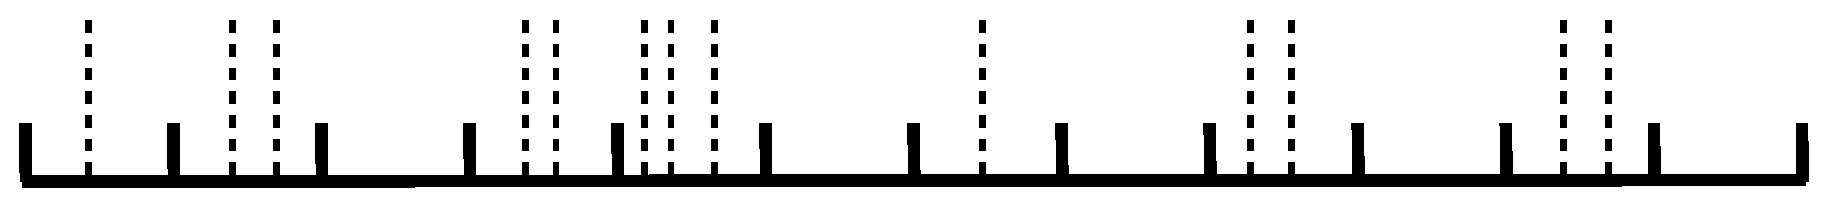
\includegraphics[width=0.6\columnwidth]{fig/motionSensorData}
\caption[Illustration of motion sensor data]{The solid lines indicate one minute
intervals and the dotted lines indicate when sensor data was collected from a
room with two motion sensors.}
\label{fig:motionSensorData}}
\end{figure}
% ----------------------------------------------------------------------------

Figure~\ref{fig:motionSensorData} illustrates an example of data collected from
a room with two motion sensors. In this example, the sensor firings in intervals
with a single sensor firing would be eliminated while the firings in intervals
with multiple sensor firings would be aggregated into a single firing as shows
in Figure~\ref{fig:filteredMotionData}.

%------------------------------------------------------------------------------
\begin{figure}[!htb]
\centering{
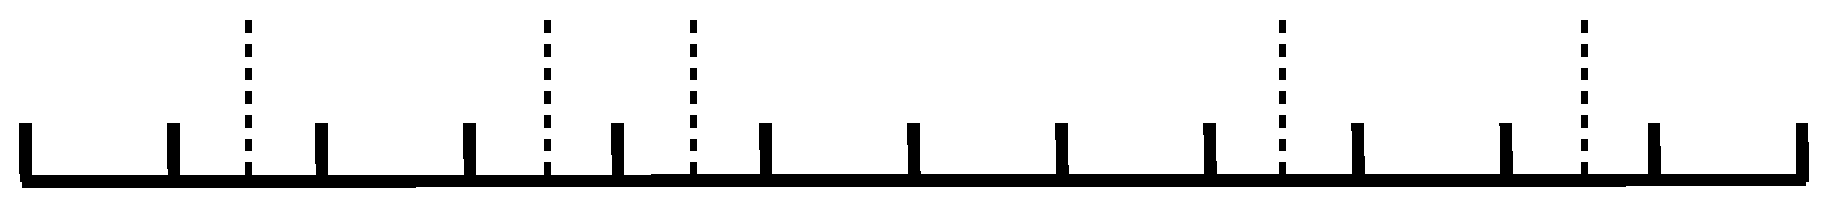
\includegraphics[width=0.6\columnwidth]{fig/filteredMotionData}
\caption[Illustration of aggregated motion sensor data]{For a room with two
motion sensors, false positive minimization removes the firings from intervals
with fewer than two sensor firings and aggregates the firings in intervals with
multiple sensor firings.}
\label{fig:filteredMotionData}}
\end{figure}
% ----------------------------------------------------------------------------

\subsubsection{Search Space Generation}

$F_A$ is scanned using moving windows and the number of aggregated firings
within the window is compared to thresholds to identify if occupancy began or
ended. The following four occupancy parameters are used to define the
beginning and ending of occupancy:
\begin{enumerate}
\item Occupancy start window size, $W_S$
\item Occupancy start firing threshold, $FT_S$
\item Occupancy end window size, $W_E$
\item Occupancy end firing threshold, $FT_E$
\end{enumerate}

$W_S$ and $FT_S$ define a frequency, $f_o$, with which the aggregated sensor
firings should occur for the room to be considered as having become occupied and
$W_E$ and $FT_E$ define a frequency, $f_v$ with which the sensors have to fire
for the room to be considered as having become vacant. If the observed frequency
of sensor firings in $F_A$ is greater than or equal to $f_o$, meaning there are
at least $FT_S$ sensor firings within a window of size $W_S$, the room is
considered to have started becoming occupied at the end of the window with
size $W_S$. If the frequency of sensor firings drops to below $f_v$, the
room will be considered to have become vacant at the end of the window with
size $W_E$. Figure~\ref{fig:occupancyStartEnd} shows an example of occupancy
start and end being identified with $W_S$ = 2 min, $FT_S$ = 2, $W_E$ = 3 min,
$FT_E$ = 2.  

%------------------------------------------------------------------------------
\begin{figure}[!htb]
\centering{
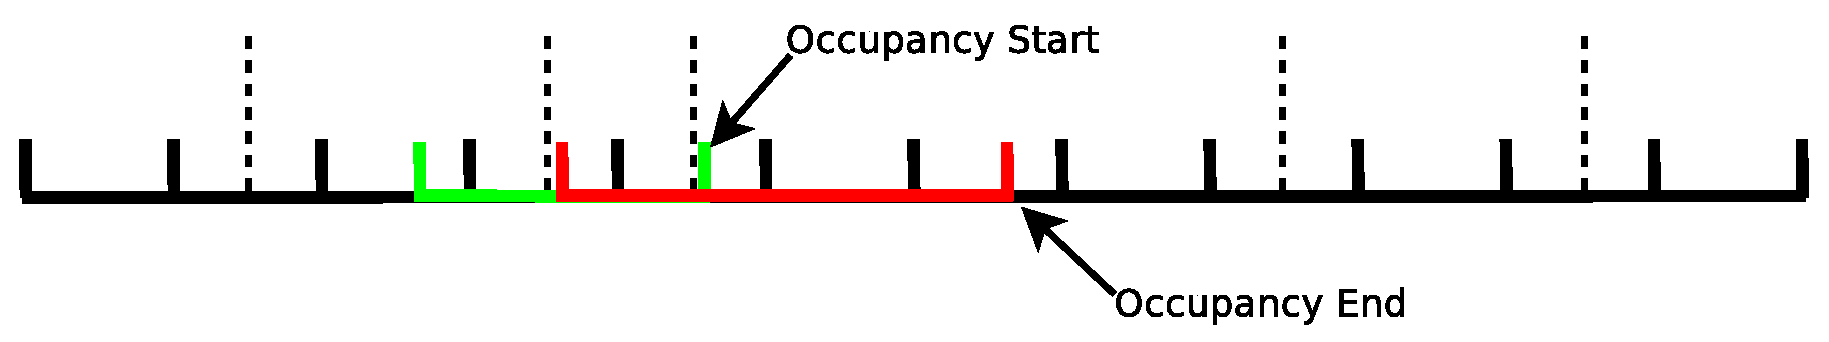
\includegraphics[width=0.6\columnwidth]{fig/searchSpaceGeneration}
\caption[Searching motion sensor data for room occupancies and vacancies]{The
occupancy start window, $W_S$ is shown in green while the occupancy end window,
$W_E$, is shown in red. The times when occupancy would be considered to have
started and ended are labeled.}
\label{fig:occupancyStartEnd}}
\end{figure}
% ----------------------------------------------------------------------------

Multiple values for $W_S$, $FT_S$, $W_E$, and $FT_E$ are tried, and the
following statistics collected for each set of parameters:
\begin{enumerate}
\item False Negative count, {\em FN}: number of sensor firings that are ignored 
\item Occupancy period, $T_O$: total amount of time a room is considered occupied
\item Occupancy transitions, $OT$: number of times a room transitions
  between being occupied and unoccupied
\item 25th percentile period $T25$: the minimum $T_O$ for at least 25\% of
  all occupancy durations in the data set 
\end{enumerate}

The output of the search space generation process is a set of occupancy
parameters, $OP$, and corresponding statistics. The parameter selection function
searches over the statistics to identify parameters that can distinguish stable
occupancy from transitional occupancy.

\subsubsection{Parameter Selection}
\label{sec:paramExt}

In order to identify optimal parameters for occupancy assessment, the parameter
selection algorithm first prunes the search space of statistics using the
following three thresholds:
\begin{enumerate}
\item Maximum number of false negatives, $FN_{max}$
\item Maximum number of occupancy transitions, $OT_{max}$
\item Maximum 25th percentile period, $T25_{max}$
\end{enumerate}

Two sets of these three parameters are defined, one for stable occupancy and one
for transitional occupancy as shown in Table~\ref{table:pruningParams}. These
parameters were selected to address the issues described in
Section~\ref{sec:occupancyAssessmentChallenges}. In order to minimize short
cycling, a longer $T25_{max}$ for stable occupancy was defined and $OT_{max}$
was defined to be small. With these restrictions, $FN_{max}$ was increased to
allow the algorithm some flexibility in selecting parameters. For transitional
occupancy, false negatives were a concern since the aim of transitional
occupancy is to capture occupancy in passageway rooms and during short-term room
usage. Thus, the threshold for $FN_{max}$ was set very low and the threshold for
$OT_{max}$ was made high since there would be many transitional occupancy events
during a day. Finally, a short duration for $T25_{max}$ was defined in order to
capture the short periods of time when passageway and short-term rooms are in
use.

\begin{table}[!htb]
\centering
\begin{minipage}{\columnwidth}
\centering
\begin{tabular}{|l|c|c|c|}
\cline{2-4}
\multicolumn{1}{c|}{}&$FN_{max}$&$OT_{max}$&$T25_{max}$ (min)\\
\hline
Stable&30&4&30\\
\hline
Transitional&4&30&3\\
\hline
\end{tabular}
\end{minipage}
\smallskip
\caption[Threshold used to search for occupancy parameters]{Parameters selected
for search space pruning reflect the characteristics of stable and transitional
occupancy.}
\label{table:pruningParams}
\end{table}

Once the search space is pruned, the remaining parameters in $OP$ form the set
of $candidateParameters$. This set is searched for the parameters that have the
minimum total occupancy time, $T_O$. This stage of the algorithm outputs two
sets of occupancy parameters, one to identify stable occupancy and one to
identify transitional occupancy. Algorithm~\ref{alg:paramSelection} describes
the parameter selection process.

\begin{algorithm} [!htb]                     % enter the algorithm environment
\caption{Parameter Selection}          % give the algorithm a caption
\label{alg:paramSelection}                           % and a label for \ref{} commands later in the document
\begin{algorithmic}                    % enter the algorithmic environment
\FOR{$i = 1:length(params)$}
\IF{$params(i, 1) / numDays < FN \: \AND \: params(i, 2) / numDays < K
  \: \AND \: params(i, 3) \geq T_{25}$}
\STATE $candidateParameters.append(params(i, :))$
\ENDIF 
\ENDFOR
\STATE $minOccupiedDurationIndex = find(min(candidateParameters(:, 4)))$
\STATE $selectedParameters.append(candidateParameters(minOccupiedDurationIndex, 5:end))$
\end{algorithmic}
\end{algorithm}

Using the parameters selected by Algorithm~\ref{alg:paramSelection} to process
sensor readings for a house over a period of ten days produces the occupancy
patterns as depicted in Figure~\ref{fig:occupancyType}. It is clear that
transitional occupancy captures frequent occupancy changes as detected by
aggregated sensor firings, while stable occupancy captures long-term room usage.

%------------------------------------------------------------------------------
\begin{figure}[!htb]
\centering{
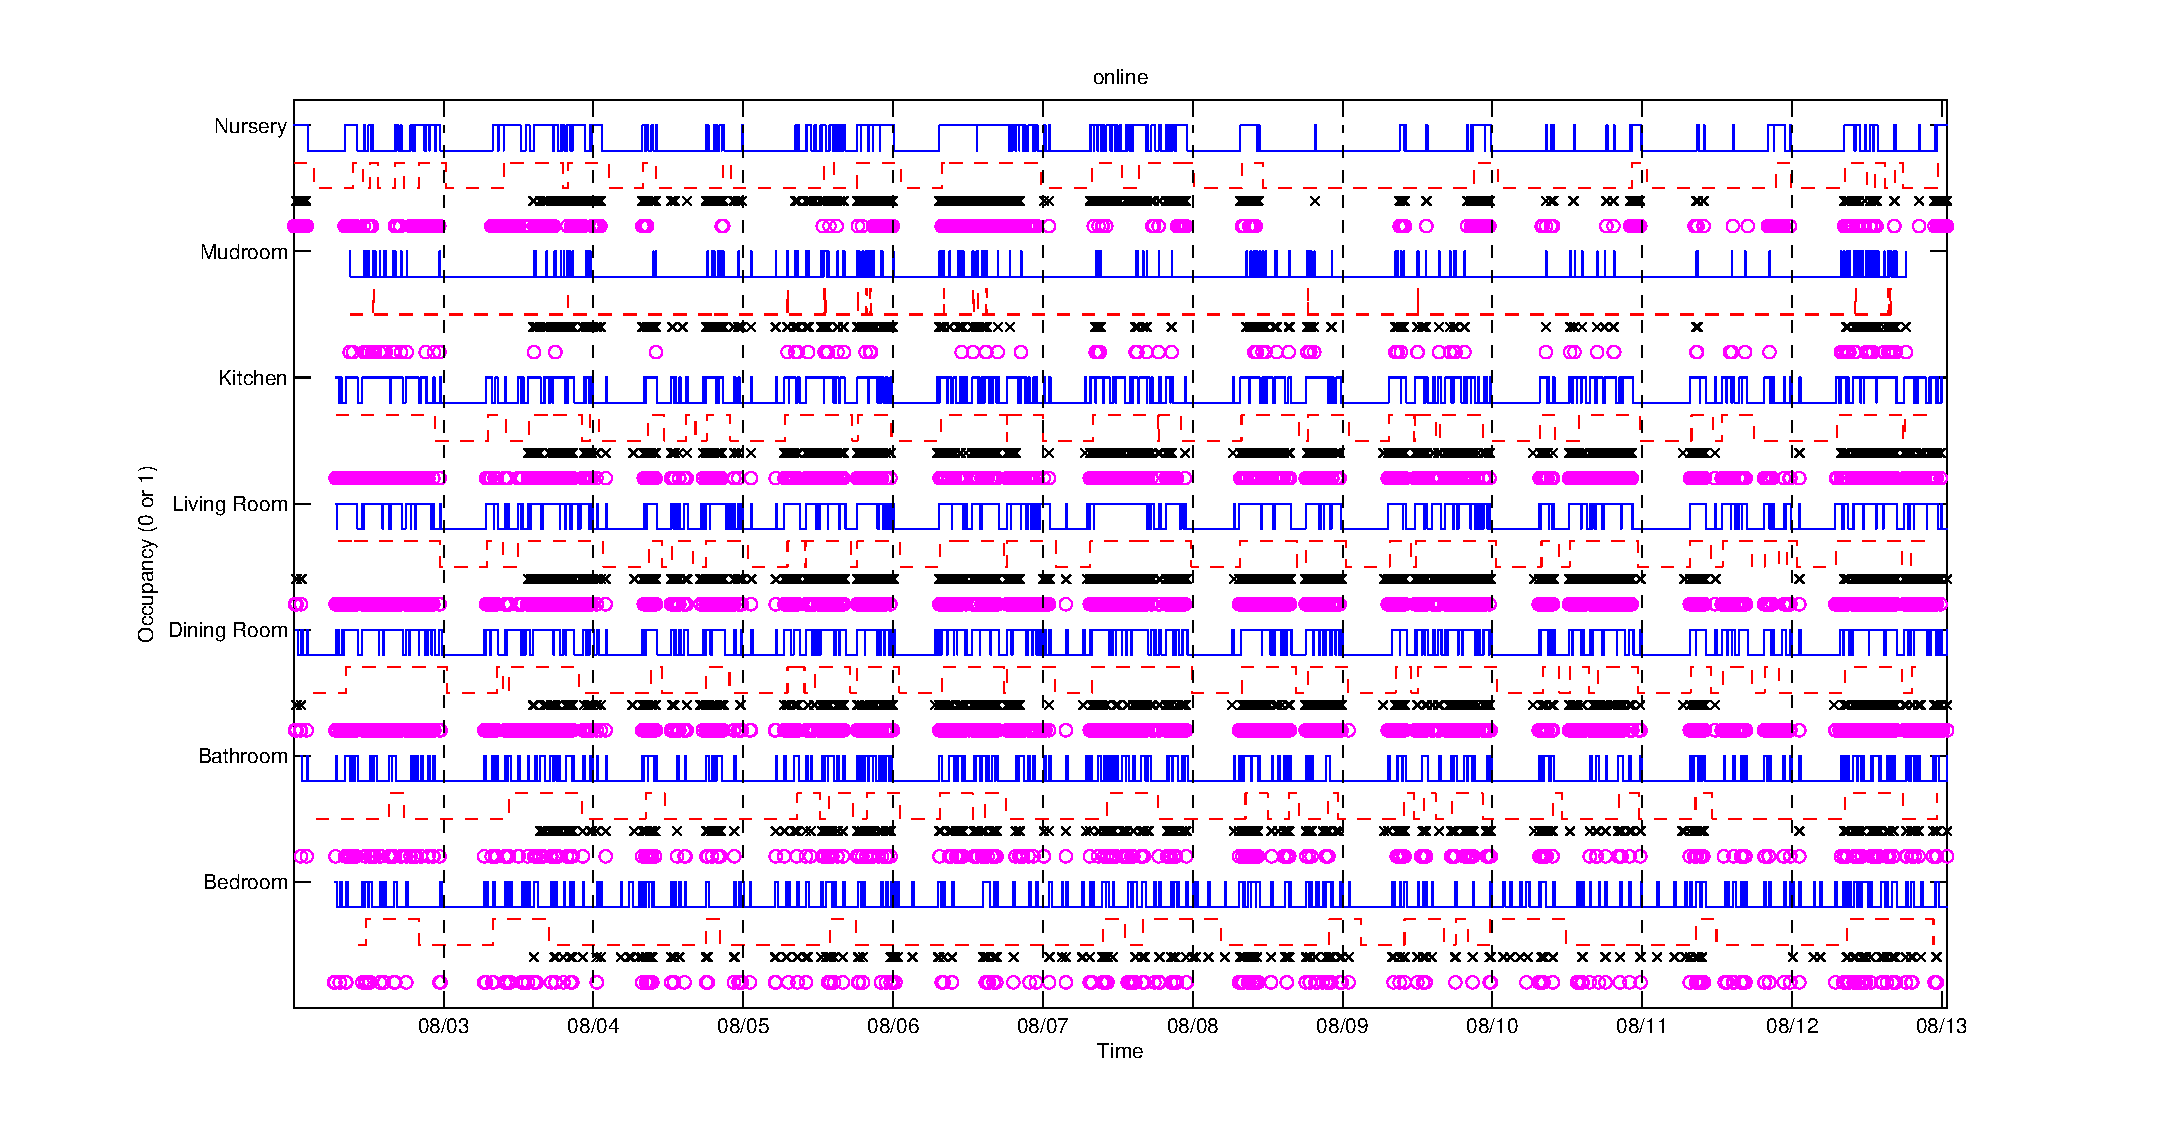
\includegraphics[width=1.0\columnwidth]{fig/occupancyTypes}
\caption[Transitional and Stable Occupancy Detected Using the Occupancy
  Model]{The solid line represents transitional occupancy, the dashed line
  represents stable occupancy, the X's depict the firings of the X10 motion
  sensors in rooms, and the O's depict the firings of the PIR sensors on
  doorways.}
\label{fig:occupancyType}}
\end{figure}
% ----------------------------------------------------------------------------

\section{Zone Control}
\label{sec:zoneControl}

After occupancy assessment, the next stage carried out by RoomZoner is hardware
control, or {\em zone control}. This involves deciding on and actuating the HVAC
system with appropriate parameters and opening, or closing, the appropriate
dampers in order to direct conditioned air through the house. In this section
the goals of zone control, the challenges that have to be overcome in
implementing it, and the actual implementation are described.

\subsection{Goals}
\label{sec:zoneControlGoals}

%% - Condition only when used
%%  - ``Occ'' -> ``On''
%%  - ``Unocc'' -> ``Off''

Since RoomZoner attempts to minimize the energy wasted in conditioning unused
rooms, the goal of zoning control is to only condition rooms when they are
used. In the ideal case this can be achieved by turning on the equipment
conditioning a room when the room is occupied and turning it off when the room
becomes unoccupied. Yet, this is complicated when implementing room-level zones
using a centralized HVAC system. 

%% - But, zones are not independent

The first complication arises due to the thermal dependence between
rooms. Houses are not designed with rooms being thermally isolated because it is
conditioned by a single piece of equipment and the flow of air from all the
rooms towards a thermostat and return vent is desired. Thus, when attempting to
zone a house at the room level, it is necessary to take into consideration the
thermal interaction between dynamically generated zones.
 
%% - Single piece of equipment

Using a single piece of equipment, instead of heating and cooling units that can
be manipulated for each room individually, such as window air-conditioning
units, complicates zoning control because the fine-grained equipment control
that is necessary for room-level zoning cannot be easily achieved. A room-level
unit cannot be turned on or off as a resident enters or leaves a room and the
effect, across multiple rooms, of actuating the HVAC system has to be taken into
consideration. 

%% - How to control equipment based on multiple conflicting zone states

Finally, a zone control algorithm has to make decisions on equipment actuation
based on multiple conflicting zone states. For instance, a particular occupied room could
be too hot or too cold while another occupied room has to be conditioned, or one
room may require stage 2 conditioning, due to it being further away from the
setpoint than another room that requires stage 1 conditioning. The zone control
algorithm has to decide between these conflicting requirements while attempting
to minimize energy consumption without compromising occupant comfort. Due to the
above constraints of room-level zoning using a single piece of equipment, a
sophisticated zone controller is necessary to achieve the goal of conditioning
rooms only when used. 

\subsection{Challenges}
As was briefly pointed out above, zone control for room-level zoning using a
centralized HVAC system is challenging. This section describes some of the
challenges that have to be overcome in implementing the zone controller for
RoomZoner.

%% - Interdependence between zones

\subsubsection{Interdependence Between Zones}

The first challenge is the interdependence between zones which is caused by all
the rooms sharing the same network of HVAC ducts. Thus, opening and closing
certain ducts, using dampers, has an effect on the airflow through other
ducts. For instance, if two rooms are services by branching ducts off a common
trunk duct, closing off one of the rooms would increase the airflow rate into
the other room. Thus, knowing the effect of closing various combinations of
dampers is essential in deciding on dynamic zones. A simple solution would be to
know the layout of ducts in the house being retrofitted, but this may not always
be known by the homeowners. Therefore, a method based on airflow measurements
from the registers, which can be easily taken using a handheld airflow meter, is
presented.

%% - Minimum airflow

\subsubsection{Minimum Airflow}
\label{sec:minAirflow}

The centralized HVAC system poses a challenge to room-level zoning and one of
the major reasons for this is the minimum airflow requirement for forced-air
HVAC systems. These systems rely on forcing air over a condensation coil,
transferring heat between the refrigerant and the air, and then delivering the
air through a series of ducts to the rooms of a house. HVAC systems are rated
for a certain output airflow depending on the operating stage. For instance, the
HVAC system in the house where the experiments were carried out produces 830
$ft^3$/min (CFM) of conditioned air when cooling in stage 1, 1200 CFM of air
when cooling in stage 2, etc. Ducts are usually properly sized so that most of
the air delivered by the fan exits the ducts, which prevents pressure buildup
within the ducts, and enables a constant flow of air over the coil. Ducts are
also sized to distribute air to rooms depending on the size of the room, with
larger rooms having more registers and wider ducts than smaller rooms.

Room-level zoning requires these ducts to be closed which decreases the amount
of air that can leave the ducts through the registers. This causes leakage
through openings such as insufficiently insulated joints and could even cause
pressure buildup within the ducts that slows down the flow of air over the
coil. This {\em back-pressure} could damage the compressor due to insufficient
thermal flow between the refrigerant and air causing the refrigerant to not
fully vaporize before flowing back into the compressor. Thus, ensuring a minimum
airflow out of the registers when deciding on which dampers to close is a
challenge that has to be overcome to ensure equipment safety.

Zoning a centralized HVAC system involves closing ducts so that air only flows
to a subset of a house. If too many ducts are closed, or ducts are closed in a
wrong configuration, back-pressure could build up resulting in energy wastage
due to leakage and equipment damage. In order to enable room-level zoning of a
centralized HVAC system the buildup of back-pressure has to be taken into
consideration when making actuation decisions.

\subsubsection{Short Cycling}
Manufacturers recommend a minimum time for which an HVAC system should operate
at a particular stage before transitioning to a lower stage, for instance
transitioning from stage 2 to stage 1 or turning off from stage 1. Transitioning
before this minimum threshold increases the wear and tear on the equipment due
to it cycling more frequently and doesn't allow the pressure to equalize between
cycles. Therefore, in implementing a system that controls the HVAC equipment at
a fine granularity, it is essential that the compressor is not short
cycled. This adds another factor to be considered when making actuation
decisions.

%% - Efficiency dependence
%%   - 2 rooms open > 1 room open
%%   - If smaller than load, BAD

\subsubsection{Efficiency Dependence}
\label{sec:efficiencyDependence}

%------------------------------------------------------------------------------
% Figure 5
\begin{figure}[!htb]
\centering{
\includegraphics[width=0.6\columnwidth]{fig/stage_energy_lagtime}
\caption[Energy Efficiency and Lag Time for HVAC Heating Stages]{Energy
  efficiency and lag time vary among the multiple stages of HVAC.}
\label{fig:multistage}}
\end{figure}
% ----------------------------------------------------------------------------

The minimum airflow requirement makes selecting an efficient HVAC stage
challenging because there is a dependence between efficiency and airflow rate. As
Figure~\ref{fig:multistage} shows, stage 2 heating is the most energy efficient
stage for heating a room by one degree. Yet, as Table~\ref{table:stageAirflow}
shows, this stage produces conditioned air at a higher rate than stage 1
heating. Due to this, more rooms have to be open for stage 2 to be
usable. Therefore, a challenge for zone control is making this trade-off between
using efficient HVAC stages and minimizing the load on the selected stage so
that the rooms being conditioned reach the setpoint faster. 

\begin{table}[!htb]
{
  \begin{tabular}{|l|c|} \hline
    Stage & Air Output Rate (CFM) \\ \hline\hline
    Stage 1 Cool & 830
    \\ \hline
    Stage 2 Cool & 1200
    \\ \hline
    Stage 1 Heat & 775
    \\ \hline
    Stage 2 Heat & 1200
    \\ \hline
    Stage 3 Heat & 775
    \\ \hline
    \end{tabular}}
\caption[Conditioned Air Output for Different Heating and Cooling
  Stages]{Conditioned Air Output for Different Heating and Cooling Stages.}
\label{table:stageAirflow}
\end{table}

%% - thermal transfer

\subsubsection{Thermal Transfer}
\label{sec:thermalTransfer}
Thermal transfer between rooms has to be taken into consideration when deciding
on rooms to be conditioned at any given time. For instance, in a house with an
open floor-plan with the kitchen and living room sharing a large opening between
them, attempting to condition the living room and not the kitchen, or vice
versa, would cause a wastage in energy due to the large amount of leakage of
conditioned air from the conditioned room to the unconditioned room. In such a
situation maintaining dependent rooms at a temperature close to the rooms being
conditioned would reduce the energy wastage by decreasing the temperature
gradient between the rooms. Thus, identifying these inter-dependencies is a
challenge that has to be addressed for zone control.

\subsubsection{Zone Coordination}
The biggest challenge to implementing room-level zoning using a centralized HVAC
system is coordinating the conditioning of zones so that energy is not wasted by
the compressor constantly being in operation or air leaking between conditioned
and unconditioned zones. RoomZoner attempts to minimize the inefficiency
by conditioning thermally homogeneous zones together so that the temperature
gradient within such zones is relatively small. This would reduce the amount of
leakage out of conditioned rooms and minimize the amount of time the HVAC system
has to be turned on when an unoccupied room is occupied because it would be
close in temperature to the neighboring rooms and, thus, can quickly be brought
to the setpoint after which the compressor can be turned off.

\subsection{Approach}
%% - Minimize system state changes 
%%  - Maximize stability

The zone controller used by RoomZoner attempts to maximize the
stability of the system by minimizing the number of system changes. Thus, at any
decision point RoomZoner attempts to maintain the damper and HVAC
equipment at their current state unless changing their state would greatly
decrease the estimated energy used, or leaving the system at its current state
would considerably affect resident comfort.

%------------------------------------------------------------------------------
\begin{figure}[t]
\centering{
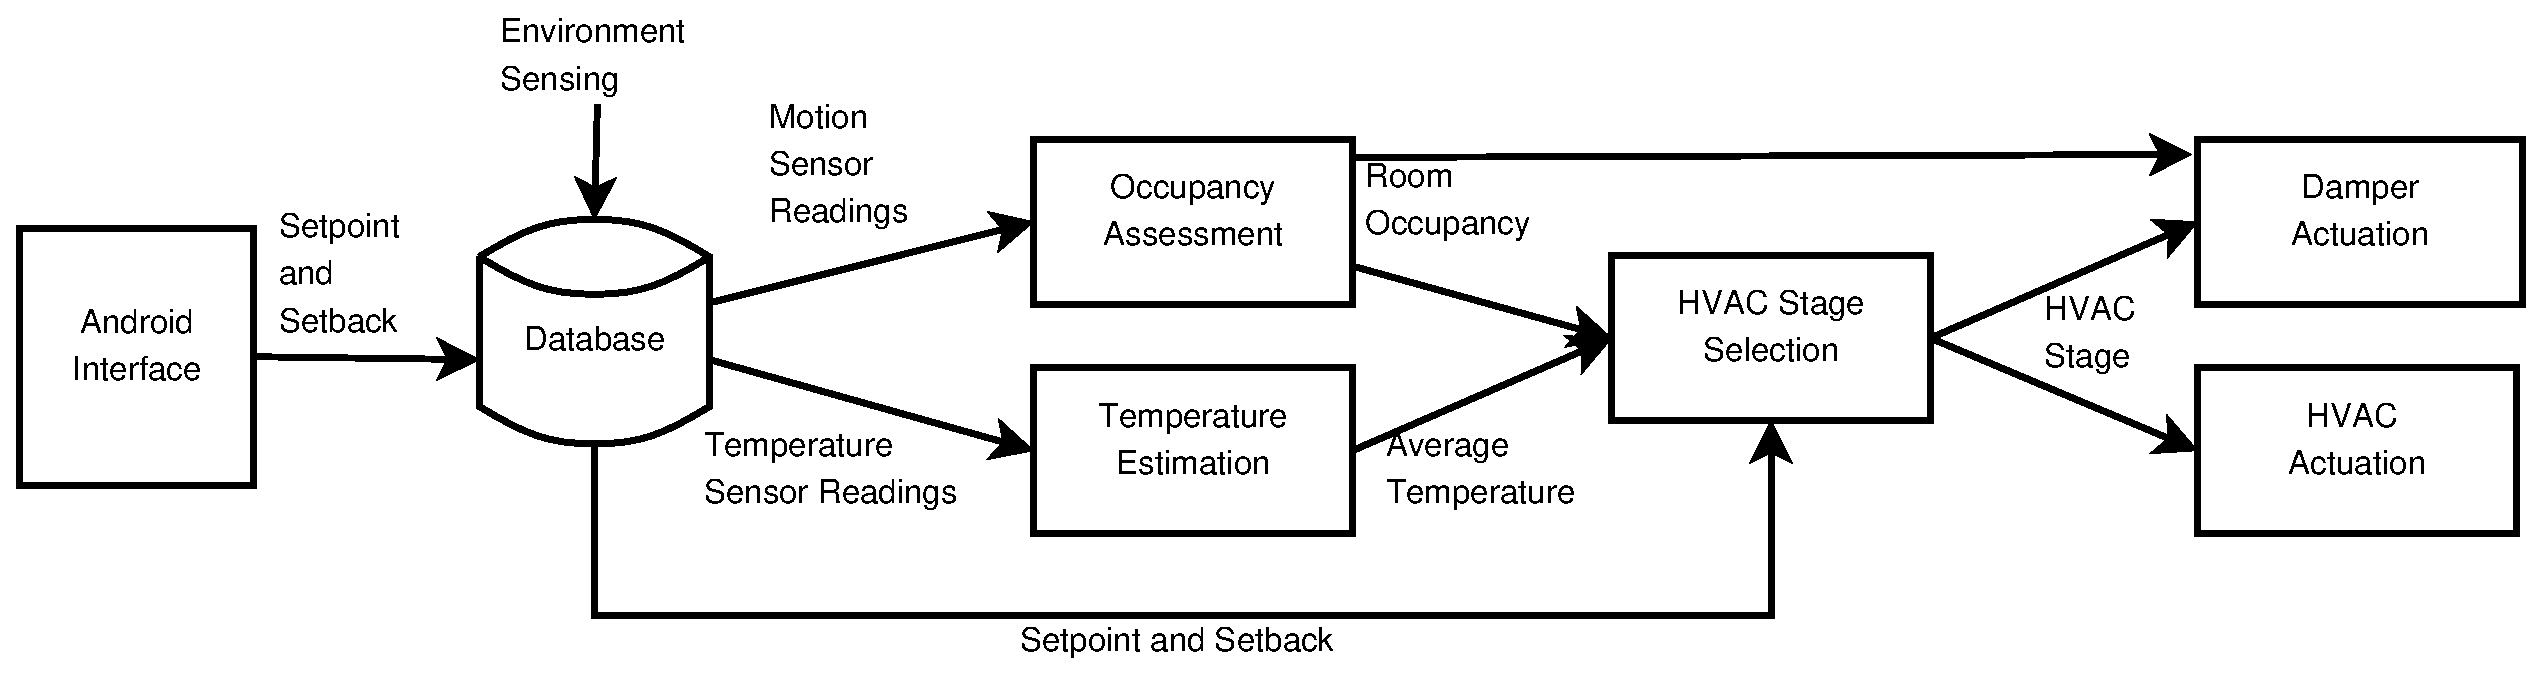
\includegraphics[width=0.9\columnwidth]{fig/controlFlow}
\caption[Zone Control Data Flow Diagram]{The data flow through the zone control algorithm.}
\label{fig:zoneControl}}
\end{figure}
% ----------------------------------------------------------------------------

Figure~\ref{fig:zoneControl} shows the main modules that encompass the zone
controller and the flow of data through the system. All sensor readings, from
temperature and occupancy sensors, are written to a database in real-time. The
database also holds the setpoint and setback temperature as input by the
resident through an Android smartphone-based user interface
(Figure~\ref{fig:android}). These values are read from the database by the zone
controller and used to assess occupancy, as described in
Section~\ref{sec:occupancyAssessment} and estimate an average temperature as
will be described in Section~\ref{sec:temperatureEstimation}. The room occupancy
results and average temperature are used to decide upon the HVAC stage to be
used when actuating the HVAC equipment. The HVAC stage decide upon, along with
the room occupancy assessment results, are used to decide on the dampers to
actuate.

%------------------------------------------------------------------------------
\begin{figure*}[!htb]
\centering{
  \includegraphics[width=0.4\columnwidth]{fig/android}
} \caption{Android smartphone-based user interface to HVAC controller.} 
\label{fig:android}
\end{figure*}
%------------------------------------------------------------------------------

\subsubsection{Temperature Estimation}
\label{sec:temperatureEstimation}
There are a number of temperature averages that could be used to control a
room-level zoned HVAC system such as the following:
\begin{enumerate}
\item Occupied room average, $t_O$: the average temperature of all rooms in use
\item Conditioned room average, $t_C$: The average temperature of rooms with open dampers
\item Whole house average, $t_H$: the average temperature of all rooms in the house
\end{enumerate}
Yet, controlling a room-level zoned HVAC system using each of these averages
individually is not ideal due to the following reasons. The occupied room
average, $t_O$ can change every time a resident enters a room or leaves a
room. This could cause a high variability in the average temperature used for
making control decisions, which could result in {\em thrashing}: the system
state changing frequently. If the newly occupied room hasn't been used recently,
it could have drifted far from the setpoint. Adding that room to the set of
rooms for which the average is calculated could cause the average temperature to
shift drastically resulting in a higher HVAC stage being requested. If the
resident leaves the room and enters a room at the setpoint, the average
temperature could again change by a large amount causing a lower HVAC stage to
be requested or the system to be turned off. Such fluctuations in HVAC control
is inefficient in terms of energy usage and could be damaging to the HVAC
hardware. Using only conditioned rooms could result in unconditioned rooms
drifting far from the setpoint so that when they become occupied a large amount
of energy would have to be expended to condition them to the setpoint. This
could be more inefficient than maintaining their temperature closer to the
setpoint even when they are unoccupied. Also, bringing these rooms towards the
setpoint could take longer, discomforting the residents. Finally, using the
average temperature of the whole house would result in the greatest stability in
terms of temperature, but this could affect the responsiveness of the
system. For instance, the average temperature of the house could be at the
setpoint if most rooms are at, or above, the setpoint. But, a particular room
could still be below the setpoint. This could be because the room is small and
has fewer air vents causing it to receive less conditioned air, it being less
well insulated than the other rooms, or it receiving a large amount of sunlight
due to its location. A resident entering such a room could be discomforted and
the system would be unable to detect it due to the other rooms skewing the
average temperature towards the setpoint.

\begin{algorithm}[!htb]                      % enter the algorithm environment
\caption{Temperature Estimation}          % give the algorithm a caption
\label{alg:temperatureEstimation}% and a label for \ref{} commands later in the document
\begin{algorithmic}                    % enter the algorithmic environment
\STATE $wholeHouseTempSum = 0$
\STATE $numRooms = 0$
\FOR{$room in rooms$}
\STATE $wholeHouseTempSum += room.temperature$
\STATE $numRooms += 1$
\ENDFOR
\STATE $wholeHouseAvg = wholeHouseTempSum / numRooms$

\STATE $conditionedRoomsTempSum = 0$
\STATE $numConditionedRooms = 0$
\FOR{$room in rooms$}
\IF{$room.damperClosed == False \: \AND \: room.transitionallyOccupied ==
  False$}
\STATE $conditionedRoomsTempSum += room.temperature$
\STATE $numConditionedRooms += 1$
\ENDIF
\ENDFOR
\STATE $conditionedRoomsAvg = conditionedRoomsTempSum / numConditionedRooms$

\STATE $occupiedRoomsTempSum = 0$
\STATE $numOccupiedRooms = 0$
\FOR{$room in rooms$}
\IF{$room.stablyOccupied$}
\STATE $occupiedRoomsTempSum += room.temperature$
\STATE $numOccupiedRooms += 1$
\ENDIF
\ENDFOR
\STATE $occupiedRoomsAvg = occupiedRoomsTempSum / numOccupiedRooms$
\IF{$mode == 'cool'$}
\STATE $averageTemp = min(wholeHouseAvg, conditionedRoomsAvg,
occupiedRoomsAvg)$
\ELSE
\STATE $averageTemp = max(wholeHouseAvg, conditionedRoomsAvg,
occupiedRoomsAvg)$
\ENDIF
\end{algorithmic}
\end{algorithm}

In order to minimize the shortcoming of each of the average temperature
calculation methods, RoomZoner uses a hybrid of all three averages to make
control decisions. Algorithm~\ref{alg:temperatureEstimation} shows the hybrid
approach adopted by RoomZoner. When heating, RoomZoner uses the maximum of the
three temperatures while when cooling it uses the minimum of the three. This
approach reduces temperature variance and increases system stability. 

\subsubsection{HVAC Stage Selection}
\label{sec:hvacStageSelection}
The HVAC stage selection process take the following inputs and decides upon the
stage with which the HVAC should be actuated:
\begin{enumerate}
\item Room occupancies
\item Average Temperature
\item Setpoint temperature
\item Setback temperature
\end{enumerate}
RoomZoner uses a hysteresis algorithm similar to the one used by Dual-Zone in
order to increase system stability. RoomZoner uses a state machine with three
states, excluding the initialization state, instead of four states as used by
Dual-Zone. This was because the custom thermostat implemented for RoomZoner
allowed individual HVAC stages to be called instead of relying on the
manipulation of setpoints on a traditional thermostat as was done by Dual-Zone.
Figure~\ref{fig:fsm} shows the state machine used by RoomZone to implement
hysteresis. The initialization state is defined as $-1$, and $0$ indicates the
HVAC system being turned off. States $1$ and $2$ correspond to the HVAC stages
described in Section~\ref{sec:efficiencyDependence}. The asymmetric transitions
between states, for example the transition from Off to Stage 1 requiring a
temperature difference of 0.7 degrees while the transition from Stage 1 to off
requiring a difference of only 0.5 degrees, provides a 0.2 degree dead-band to
prevent rapid fluctuations between the two states.

%------------------------------------------------------------------------------
\begin{figure}[!htb]
\centering{
\includegraphics[width=0.9\columnwidth]{fig/stateMachine}
\caption[Finite-State Machine Used for HVAC Stage Selection.]{The finite-state
  machine which provides hysteresis during the stage selection process.}
\label{fig:fsm}}
\end{figure}
% ----------------------------------------------------------------------------

Algorithm~\ref{alg:hvacStageSelection} shows how hysteresis is used to select an
HVAC stage. RoomZoner compares the average temperature generated by
Algorithm~\ref{alg:temperatureEstimation} to the setpoint if the house is
occupied. Otherwise, it compares the average temperate to the setback.

\begin{algorithm}[!htb]                      % enter the algorithm environment
\caption{HVAC Stage Selection}          % give the algorithm a caption
\label{alg:hvacStageSelection}% and a label for \ref{} commands later in the document
\begin{algorithmic}                    % enter the algorithmic environment
\IF{$numOccupiedRooms > 0$}
\STATE $tempDiff = averageTemp - setpoint$
\ELSE
\STATE $tempDiff = averageTemp - setback$
\ENDIF

\IF{$mode == 'heat'$}
\STATE $tempDiff = -tempDiff$
\ENDIF

\IF{$hvacStage == -1$}
\IF{$tempDiff >= 1.7$}
\STATE $hvacStage = 2$
\ELSIF{$tempDiff > 0.5$}
\STATE $hvacStage = 1$
\ELSE
\STATE $hvacStage = 0$
\ENDIF
\ELSIF{$hvacStage == 0$}
\IF{$tempDiff > 1.7$}
\STATE $hvacStage = 2$
\ELSIF{$tempDiff > 0.7$}
\STATE $hvacStage = 1$
\ENDIF
\ELSIF{$hvacStage == 1$}
\IF{$tempDiff > 1.7$}
\STATE $hvacStage = 2$
\ELSIF{$tempDiff < -0.5$}
\STATE $hvacStage = 0$
\ENDIF
\ELSE
\IF{$tempDiff < -0.5$}
\STATE $hvacStage = 0$
\ELSIF{$tempDiff < 0.3$}
\STATE $hvacStage = 1$
\ENDIF
\ENDIF
\end{algorithmic}
\end{algorithm}

\subsubsection{Damper Actuation}
\label{sec:damperActuation}

%% - Open all ``occ''
%%  -> no room-level temperature control

Damper actuation involves selecting the dampers to be opened and closed and
sending the appropriate commands to the damper control circuitry. Since the zone
controller does not use room-level temperature control all rooms that are
occupied have their dampers open. The HVAC stage selected by
Algorithm~\ref{alg:hvacStageSelection} determines the minimum airflow into the
rooms in order to ensure equipment safety. The damper actuation module attempts
to ensure this minimum airflow by strategically opening additional rooms as
needed so that there is minimum impact to the efficiency with which the occupied
rooms are conditioned. The decision that has to be made is on what additional
rooms, called {\em dump rooms}, that comprise the {\em dump zone} have to be
opened, if they are closed. This decision is based on ensuring the safety of the
HVAC equipment by minimizing the chance of back-pressure buildup due to too many
dampers being closed.

%% - dump when needed
%%  - dump zones based on thermal transfer
%%    - not temp

%% - keep old occupied rooms as dump zones

Algorithm~\ref{alg:dumpZoneSelection} is used during zone control to select the
rooms that comprise the dump zone. Whenever there are insufficient rooms
occupied in order to ensure sufficient airflow out of the ducts, the dump zone
selection algorithm is called. This algorithm selects dump zones based on the
estimated benefit, in terms of thermal transfer, to the occupied rooms rather
than the actual temperatures of the potential dump rooms. Also, the algorithm
prefers rooms that have been occupied in the near past as dump rooms. These
approaches to dump zone selection ensures the zone controller is able to achieve
its goal of maximizing system stability by minimizing state changes.

\begin{algorithm}[!htb]                      % enter the algorithm environment
\caption{Dump Zone Selection}          % give the algorithm a caption
\label{alg:dumpZoneSelection}% and a label for \ref{} commands later in the document
\begin{algorithmic}                    % enter the algorithmic environment
\FOR{$room in rooms$}
\STATE $activeRooms = []$
\STATE $dumpCandidate = []$
\IF{$room.stageRequest > 0 \: or \: room.transitionallyOccupied$}
\STATE $activeRooms.append(room)$
\ELSE
\STATE $dumpCandidates.append(room)$
\ENDIF
\ENDFOR

\STATE $dumpSets = []$

\FOR{$dumpSet in combinations(dumpCandidates)$}

\STATE $airflow = calculateAirflow(activeRooms, dumpSet)$

\STATE $minFlowChange = INF$
\FOR{$room in dumpSet$}
\IF{$room.openAirflow < minflow$}
\STATE $minFlowChange = room.openAirflow - room.closedAirflow$
\ENDIF
\ENDFOR

\IF{$airflow > safeAirflow \: \AND \: minFlowChange > airflow - safeAirflow$}
\STATE $dumpSets.append(dumpSet)$
\ENDIF

\ENDFOR

\STATE $bestEnergy = -INF$; $bestChanges = 0$; $bestDumpZone = []$
\FOR{$dumpSet in dumpSets$}

\STATE $inactiveRooms = rooms$
\FOR{$room in activeRooms$}
\STATE $inactiveRooms.remove(room)$
\STATE $activeZoneEnergy += voltages(hvacStage, dumpSet, room)$
\ENDFOR

\STATE $damperChanges = 0$
\FOR{$room in dumpSet$}
\STATE $inactiveRooms.remove(room)$
\IF{$room.damperClosed$}
\STATE $damperChanges += 1$
\ENDIF
\ENDFOR

\FOR{$room in inactiveRooms$}
\IF{$room.damperClosed == False$}
\STATE $damperChanges += 1$
\ENDIF
\ENDFOR

\IF{$activeZoneEnergy - damperCost * damperChanges > bestEnergy -
  damperCost * bestChanges$}
\STATE $bestDumpZone = dumpSet$
\STATE $bestEnergy = activeZoneEnergy$
\STATE $bestDamperChanges = damperChanges$
\ENDIF

\ENDFOR

\STATE $dumpZone = []$
\FOR{$room in bestDumpZone$}
\STATE $dumpZone.append(room)$
\STATE $estimatedAirflow = calculateAirflow(activeRooms, dumpZone)$
\IF{$estimatedAirflow > safeAirflow$}
\STATE $return dumpZone$
\ENDIF
\ENDFOR

\end{algorithmic}
\end{algorithm}

The first phase of dump zone selection is separating the rooms into active
rooms, those room that require conditioning due to either being stably or
transitionally occupied or being beyond the setback temperature, and dump
candidates. Next, all combinations of dump candidates are evaluated in order to
identify the set of rooms that have the greatest positive impact on the goals of
zone control. 

% \begin{algorithm}[!htb]                      % enter the algorithm environment
% \caption{Airflow Calculation}          % give the algorithm a caption
% \label{alg:calculateAirflow}% and a label for \ref{} commands later in the document
% \begin{algorithmic}                    % enter the algorithmic environment
% \FOR{$room \: in \: rooms$}
% \IF{$room \: in \: activeRooms \: \OR \: dumpSet$}
% \STATE $airflow += room.openAirflow$
% \ELSE
% \STATE $airflow += room.closedAirflow$
% \ENDIF
% \ENDFOR
% \end{algorithmic}
% \end{algorithm}

The first step in dump candidate evaluation is estimating the total airflow out
of the ducts with a particular set of dump rooms. The airflow calculator
provides a conservative estimate of the expected airflow when a particular set
of registers is closed. This estimation is based on empirical values of airflow
collected with a airflow meter. Two values of airflow are collected for each
register: openAirflow and closedAirflow. {\em openAirflow} is the volume of air
output from a register when all registers are open, while {\em closedAirflow} is
the volume of air output from a register when it is closed while all other
registers are open. these values are used as approximations of the airflow out
of a register when it is opened or closed. They are lower bounds since if any
other register is closed concurrently, these values are expected to
increase. The total airflow is calculated by adding together either a
closedAirflow or an openAirflow value for each register in the house depending
on whether the register is closed or open. This sum provides a lower bound for
the amount of air expected to leave the ducts. This value being beyond the
safety limit of the HVAC system would ensure the safety of the hardware. A lower
bound calculation was used instead of an accurate measurement of the airflow due
to the large number of measurements necessary to build such a model. For the
residence where the system was implemented, which has 13 registers, $2^{13} =
8192$ measurements would have to be taken to build a complete model. Using the
lower bound allows the model to be built within a few hours.

The estimated airflow is used to eliminate dump candidates that would not help
with ensuring a safe volume of airflow out of the system. In addition to
ensuring that this safety limit is met, RoomZoner also verifies that no
room in the set can be removed and still have a safe airflow out of the system
using the minimum airflow change which is the minimum difference in airflow from
a room in the set being opened and closed. This minimum airflow change is
compared to the difference between the airflow estimate and the safe airflow to
ensure that the change is greater than the difference and therefore the room has
to be opened.

The final step of damper actuation is optimizing over the search space of dump
candidates that passed the airflow check. The optimization is done over two
parameters: {\em zone energy} and {\em damper changes}. Zone energy is an
estimate of the thermal impact on occupied rooms by a particular dump zone and
damper changes is the number of rooms that have to be changed from currently
being opened to closed, or closed to opened. Zone energy is calculated using
voltage values that are obtained from a circuit model of airflow in a house that
we describe in the next subsection. This model assume rooms are wires with
resistors between them and the air coming out of the dampers are current
sources. Give a set of current sources, as estimated airflows from the
registers, the model provides voltages for each room. These voltages describe
temperature changes in rooms with higher voltages indicating a greater
temperature change. Thus, the optimization function attempts to search for dump
zones that have the greatest impact on the voltage of the occupied rooms,
indicating the possibility of the greatest positive impact on those rooms in
terms of thermal transfer. With this approach we address the thermal transfer
challenge described in Section~\ref{sec:thermalTransfer}. In addition to the
zone energy, we also attempt to minimize the number of damper changes that have
to be made to achieve the dump zone. This ensures that rooms that were recently
occupied are preferred as dump candidates since their dampers are more likely to
be open and also minimizes the number of state changes necessary, as the zoning
controller is trying to achieve. Preferring recently occupied rooms helps ensure
that rooms that are used in mult-room occupancy scenarios are kept close to the
setpoint. This also helps ensure that the temperature of rooms that are more
likely to be occupied in the future, due to temporal locality, are not allowed
to drift far from the setpoint.

\subsubsection{Thermal Model}

\begin{figure}[!htb]
  \centering
  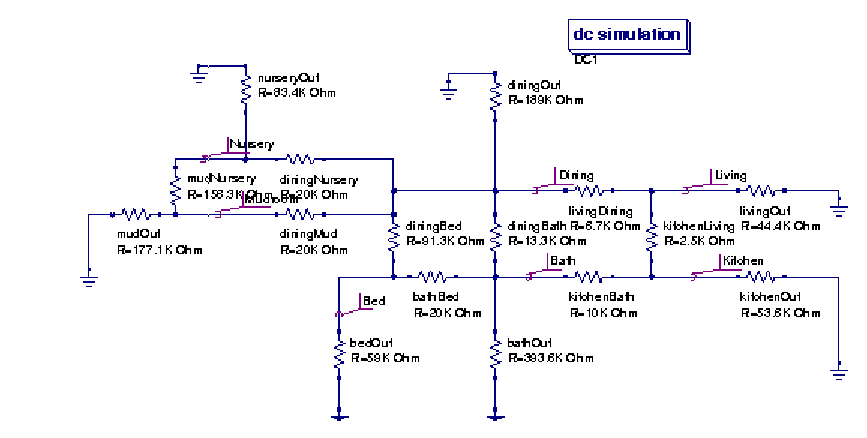
\includegraphics[width=0.8\columnwidth]{fig/houseCircuit}
  \label{fig:houseCircuit}
  \caption{Circuit model of house generated in Qucs circuit simulator.}
\end{figure}

A circuit model (Figure~\ref{fig:houseCircuit}) of the house is generated using
the Quite Universal Circuit Simulator (Qucs)~\cite{qucs}. The model is based on
the assumption that the total resistance between the house and the external
environment is 1 M$\Omega$. This total resistance is distributed across all
rooms based on the total surface area of external walls and ceilings in a room
(Table~\ref{table:extSurface}).

The 1 M$\Omega$ resistance is distributed across the rooms in an inverse
proportion to the external surface area using the following set of equations:
\begin{eqnarray*}
R_L + R_K + R_{Ba} + R_{Be} + R_M + R_N + R_D &=& 1 \mathsf{M}\Omega \\
554.03R_L = 426.75R_K = 84.6R_{Ba} = 368R_{Be} &=& \\144R_M = 233.75R_N &=&
275.25R_D
\end{eqnarray*}
Solving the set of equations above give the external resistances in
Table~\ref{table:extSurface}. 

Further, we assume a $25\,^{\circ}\mathrm{F}$ temperature difference between the interior
and exterior of the house based on observations of an ability to maintain the
temperature in the house at $70\,^{\circ}\mathrm{F}$ when the external temperature is
$45\,^{\circ}\mathrm{F}$. This $25\,^{\circ}\mathrm{F}$ is translated to a 25V potential difference
between the interior and exterior, $V_{ext}$ and current flows out of each room,
which translate into heat loss to the external environment, are calculated using
$I = V_{ext}/R$ where $I$ is the current through external walls and ceilings and
$R$ is the resistance between each room and its exterior from
Table~\ref{table:extSurface}. The heat loss, in terms of current is given in
Table~\ref{table:extSurface}.

\begin{table}[!htb]
{
  \begin{tabular}{|l|l|l|l|} \hline
    Room & Area (ft$^2$) & Resistance (K$\Omega$) & Current($\mu$A) \\ \hline\hline
    Living Room & 554.03 & 69.9 & 357.7
    \\ \hline 
    Kitchen & 426.75 & 53.8 &464.7
    \\ \hline
    Bathroom & 84.6 & 352.4 & 70.9
    \\ \hline
    Bedroom & 368 & 81 & 308.6
    \\ \hline
    Mudroom & 144 & 207 & 120.8
    \\ \hline
    Nursery & 233.75 & 127.5 & 196.1
    \\ \hline
    Dining Room & 275.25 & 108.3 & 230.8
    \\ \hline
    \end{tabular}}
\caption{Area of, resistance of, and current through external surfaces.}
\label{table:extSurface}
\end{table}

We then calculate all the currents through the circuit using Kirchhoff's
equations given a current input into the Kitchen, $I_{KI}$, which represents
airflow into the kitchen. The following set of equations are solved to get all
currents in the circuit in this steady-state scenario. The subscripts on the
current variables, $I$, indicate the source and destination of the current so
that $I_{KL}$ is a current flowing from the kitchen to the living room. The only
variable that violates this convention is $I_{KI}$ which is the input current
source into the kitchen. 

\begin{eqnarray}
I_{KI} &=& 464.7\mu + I_{KL} + I_{KBa} \\ 
I_{KL} &=& 357.7\mu + I_{LD} \\
I_{KBa} &=& 70.9\mu + I_{BaBe} - I_{DBa} \\
I_{LD} &=& 230.8\mu + I_{DBa} + I_{DBe} + I_{DM} + I_{DN} \\
I_{DBa} &=& 70.9\mu + I_{BaBe} - I_{KBa} \\
I_{DBe} &=& 308.6\mu - I_{BaBe} \\
I_{DM} &=& 120.8\mu + I_{MN} \\
I_{DN} &=& 196.1\mu - I_{MN} \\
I_{BaBe} &=& 308.6\mu - I_{DBe} \\
I_{MN} &=& 196.1\mu - I_{DN}
\end{eqnarray}

\section{Preliminary Implementations and Lessons Learned}
The initial implementation of occupancy assessment involved a simple threshold
based approach. For a room with $N$ sensors, if $N/2$ sensor firings were
recorded within a one minute interval, the room was considered to be
occupied. This was based on the assumption that if at least half the sensors in
a room fired within a short period, an actual occupancy should have been
detected within the room. 

While this approach proved sufficiently reliable to detect room occupancies, it
could not differentiate between rooms being actually occupied or sensors being
triggered as people passed through rooms. This causes the occupancy assessment
algorithm to classify occupancy as either stable or transitional based on sensor
firing characteristics.

A number of HVAC stage selection and dump zone selection algorithms were
implemented before settling on the algorithms described above. In the following
subsections some of these approaches are described.

\subsubsection{HVAC Stage Selection}
RoomZoner uses the average temperature to select an HVAC stage. Before settling
on this implementation, two alternative HVAC stage selection strategies, as
described below, were considered.

\par {\bf Majority room request. } In this scheme, each room is given a vote to
decide on an optimal HVAC stage depending on its temperature and
occupancy. Hysteresis is used on a per-room basis using the algorithm depicted
in Figure~\ref{fig:stateMachine}. Once all the rooms cast their votes, the
majority from among the votes is used to control the HVAC system. For instance,
if five of the seven rooms requested stage 1 cooling while the other two rooms
requested stage 2 cooling, the HVAC would be actuated in stage 1. 

In most instances very few rooms are far enough from the setpoint to request
stage 2 and, therefore, the HVAC system operates in stage 1 almost exclusively
when it is turned on. This results in rooms that require stage 2 heating or
cooling to not receive the appropriate volume of conditioned air and, thus, take
a long time to reach the setpoint or not be able to achieve that temperature.

\par {\bf Max room request. }
Due to the shortcomings of the majority room request HVAC stage selection
approach, the stage selector was modified to use the maximum stage request. With
this approach, if any room requires stage 2 this stage would be used to
condition all the rooms. Such an approach is based on the assumption that rooms
requiring a higher stage could reach the setpoint within a reasonable time while
rooms requiring a lower stage would reach the setpoint faster than with the
lower stage, thus saving energy.

What was observed when executing the system with the max stage request HVAC
stage selection policy was many rooms overshooting the setpoint temperature due
to them requiring less conditioned air than that provided with stage 2 heating
or cooling. This results in discomfort for residents due to rooms being too cold
or too hot.

\subsubsection{Dump Zone Selection}
RoomZoner selects dump zones based on their estimated influence on the active
rooms using a simple model of thermal flow through the house. Before
implementing this dump zone selection technique, three dump zone selection
algorithms were considered. The first one was based on room temperatures, the
second was based on a pre-defined selection priority, and the third was based on
room connectivity,.
  
\par {\bf Temperature-based dump zone selection. } In this approach, for each
room that was not occupied RoomZoner calculates the difference between
the temperature in the room and the setpoint. It then sorts these dump
candidates based on temperature difference so that rooms further away from the
setpoint get a higher priority of being selected as dump rooms than rooms closer
to the setpoint. This approach was based on the intuition that maintaining the
average temperature of the unoccupied rooms at close to the setpoint as possible
would minimize the time required to heat, or cool, these rooms when they were
occupied.

Execution of RoomZoner using this dump zone selection approach caused dump zones
to constantly fluctuate. For instance, in a particular iteration of RoomZoner if
the bathroom and a bedroom were dump candidates with only one of the two
required for the dump zone and the bathroom was further from the setpoint than
the bedroom, the bathroom would be conditioned and the bedroom left
unconditioned. In the next iteration, due to being conditioned the bathroom
would be closer to the setpoint than the bedroom causing the bedroom to be
selected as the dump room and the bathroom to be left unconditioned. Such an
approach has two drawbacks. The first is the constant alternating between rooms
could result in a room never being sufficiently heated or cooled to approach the
setpoint. Each time a room alternates from being a dump room to being left
unconditioned, the energy expended in heating or cooling that room could be lost
due to leakage. The second shortcoming of this approach is the constant opening
and closing of active registers or dampers as rooms are added and removed from
the dump zone. This could reduce the lifetime of these dampers, both in terms of
energy if they are operating on batteries, as well as the number of mechanical
actuations they are capable of sustaining.

\par {\bf Priority-based dump zone selection. } In the next attempt at dump room
selection, a pre-defined priority scheme with which rooms are added to the dump
zone was tried. The following priority scheme was utilized:
\begin{itemize}
\item Transitionally occupied rooms have a higher priority than occupied rooms.
\item Rooms with open dampers have a higher priority than rooms with closed
  dampers.
\item Rooms further from the setpoint have a higher priority than rooms closer
  to the setpoint.
\end{itemize}
This approach to dump zone selection was aimed at minimizing thrashing without
compromising occupant comfort. By preferring transitionally occupied rooms to
unoccupied rooms, rooms that are occupied, even temporarily, are kept at a
comfortable temperature. Transitionally occupied rooms are also more likely to
be stably occupied than rooms that are unoccupied for long periods of time. Thus
by maintaining them at close to the setpoint, they can be quickly and
efficiently conditioned to the setpoint in the event that residents begin using
them. By preferring rooms with dampers already opened to rooms with closed
dampers, the number of transitions between opening and closing dampers is
minimized, increasing system stability. Finally, selecting rooms further from
the setpoint than those closer to the setpoint ensures no room will drift very
far from the setpoint before it is conditioned. 

Priority-based dump zone selection resulted in very stable dump zones with
minimal thrashing, yet it also caused certain rooms to not be conditioned for
long periods of time due to being low on the priority list. When such rooms were
occupied, a large amount of energy and time was required to condition it back to
the setpoint, and occupants were uncomfortable for long durations of time while
the room warmed up or cooled down. 

\par {\bf Connectivity-based dump zone selection. } In the third attempt at a
dump zone selection algorithm, it was decided to prioritize neighboring rooms
when selecting dump zones. This approach was based on the intuition that
neighboring rooms would have the greatest influence on occupied rooms. For
instance, if a neighboring room is not conditioned, the temperature difference
between it and its occupied neighbor would be large resulting in a greater
thermal transfer between the occupied room and the neighboring room. By
conditioning neighboring rooms, this thermal gradient could be minimized
reducing the leakage. Also, leakage from a neighboring room into an occupied
room could benefit the occupied room.

Connectivity-based dump zone selection minimized fluctuations between dump rooms
since occupied rooms do not change as frequently. Due to the fact that rooms
neighboring occupied rooms are more likely to be occupied in the near future,
and these rooms are selected as dump rooms, the problem of a person entering an
unoccupied room and it being far from the setpoint was mitigated. Yet, it was
observed that this approach resulted in less conditioned air being provided to
occupied rooms. Airflow measurement experiments indicated that closing dampers
and registers within a branch of the duct system increased the pressure within
that branch and thus forced more air out of the open dampers in that
branch. Since neighboring rooms are more likely to share a common branch of the
HVAC ducts, opening neighboring rooms resulted in a lower volume of conditioned
air entering occupied rooms. The model of thermal flow attempted to capture this
phenomenon and suggest rooms that would have the greatest positive impact on
occupied rooms.

\section{Software Implementation}

In a similar approach to case study 1, RoomZoner was implemented using
Python. Some of the algorithms used in the Python implementation are presented
above. Similar to case study 1, the RoomZoner software was, also, written in
MacroLab in order to evaluate the ease with which an application written in
MacroLab could be evolved as its functionality is extended. The code in
Figure~\ref{code:cs2} shows the high level program logic. $assessOccupancy$,
$calculateAverageTemperature$, and $selectDumpZone$ are functions that can
easily be written in MacroLab.

\begin{figure}
  \begin{macrolab}
RTS = RunTimeSystem();
weatherdirect = RTS.getMotes('type', 'weatherdirect');
tempSensors = SensorVector(weatherdirect, 'temperature');
x10 = RTS.getMotes('type', 'X10');
motionSensors = SensorVector(x10, 'motion');
motionSensorIDs = uint8({[8 1 9], [2 6], [10 5], [4], [7 11], [12 14], [3 15]});
tempSensorIDs = uint8({[1 3], [2], [6 7], [4 9 11], [12 13], [5 14], [8 10]}); 
damperIDs = uint8({[3 5], [1 2], [8 4], [10], [11 15], [12 14], [5 7]});
nightStart = [0 0 0 2 0 0];
nightEnd = [0 0 0 7 0 0];
curState = 'On'
every(60000)
  mode = dbRead('zoning', 'mode', 'latest')
  damperState = dbRead('zoning', 'damper', damperIDs) 
  motionVals = motionSensors.sense();
  tempVals =  tempSensors.sense();
  [stablyOccupied, transitionallyOccupied] = assessOccupancy(motionVals, motionSensorIDs);
  aTemp = calculateAverageTemperature(tempVals, stablyOccupied, transitionallyOccupied, damperState)
  if length(stablyOccupied) > 0 || length(transitionallyOccupied) > 0
    SP = dbRead('zoning', 'setpoint', 'latest');
  else
    SP = dbRead('zoning', 'setback', 'latest');
  if mode == 'heat'
    deltaTemp = SP - aTemp;
  else
    deltaTemp = aTemp - SP;
  curState = getNextState(curState, deltaTemp);
  if curState > 0:
    dumpRooms = selectDumpZone(curState, stablyOccupied, transitionallyOccupied);
    hvacActuate(mode, curState, [stablyOccupied dumpRooms]);
  else
    hvacActuate(mode, curState, stablyOccupied);
  end
end
  \end{macrolab}
  \smallskip
  \hrule width 1\columnwidth
  \caption{MacroLab implementation of RoomZoner.}
  \label{code:cs2}
\end{figure}

\section{Evaluation}

RoomZoner is evaluated in the same house used to evaluate day/night zoning by
alternating between room-level zoning and whole house conditioning. In the
following subsections the energy measurements of RoomZoner is compared to whole
house conditioning and the lessons learned by implementing room-level zoning in
MacroLab are discussed.

\subsection{Zoning Evaluation}

To evaluate RoomZoner the control of the HVAC system is alternated between
single-zoned whole house control and room-level zoned control over a 42 day
period, such that each system ran every other day. This experimental procedure
was selected to minimize the effect of changing weather patterns on energy
statistics. The experiments with alternating RoomZoner and whole house
conditioning were carried out over a period of four months during the
winter. For this evaluation we excluded the data from days when the HVAC did not
turn on due to the temperature never being below the setpoint and days when
their were clear data loss due to unusually low energy consumption values. From
the remaining days we extracted 21 days worth of data for each system so that
for each month RoomZoner and whole-house control had the same amount of
data. This was done to ensure fairness by minimizing the effect of weather when
the data for one system is mostly from the coldest part of the winter while the
other system's data is from milder days. The energy consumed by the HVAC system
was monitored using The E-Monitor total home energy management
system~\cite{emonitor}. Figure~\ref{fig:cs2energy} shows the energy consumed in
conditioning a house using RoomZoner and whole house conditioning. This graph
indicates that whole-house conditioning consumed 14.4\% more energy than the
prototype implementation of room-level zoning, on average.

\begin{figure}[ht]
  \centering
  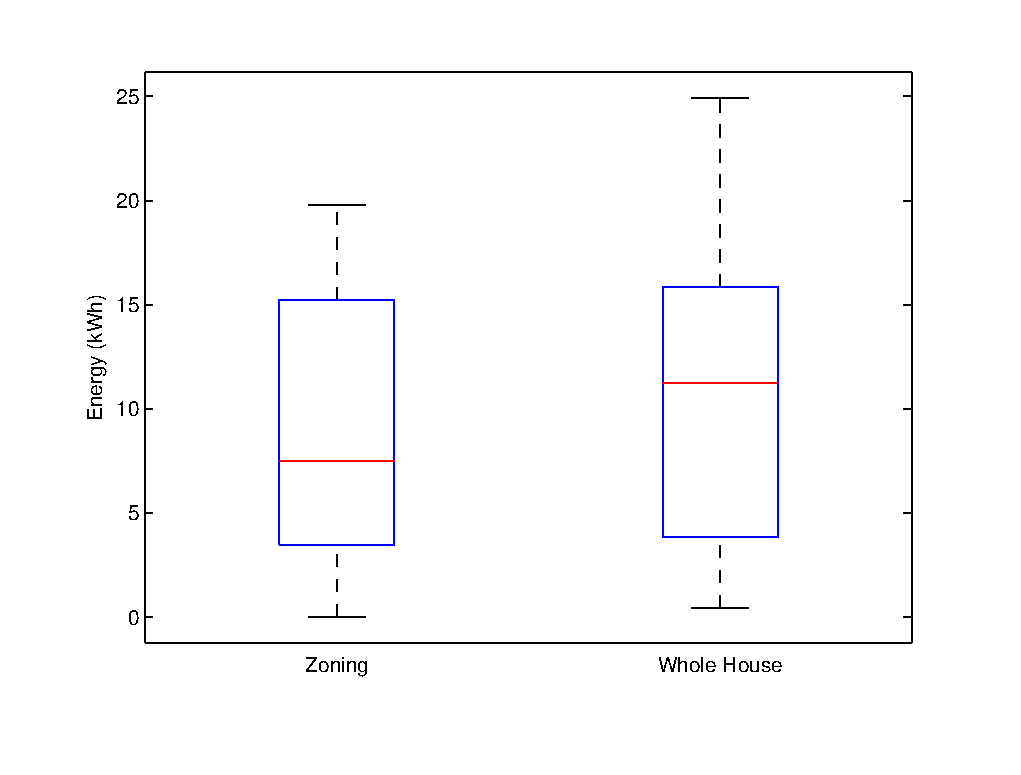
\includegraphics[width=0.6\columnwidth]{fig/cs2boxplot.eps}
  \caption[Energy usage of RoomZoner vs. whole house conditioning]{The
  implementation of room-level zoning uses 14.4\% less energy than whole house
  heating on average.}
  \label{fig:cs2energy}
\end{figure}

The energy savings for RoomZoner cannot be compared to the savings for day/night
zoning due to three reasons. The first is the day/night zoning experiments being
conducted during the summer when the HVAC system was used for cooling while the
RoomZoner experiments were conducted during the winter. The second is that the
day/night zoned system was compared against a standard residential thermostat
controlling the whole house conditioning while RoomZoner was compared against a
custom whole house conditioning system that used the same infrastructure as
RoomZoner. In whole house mode the thermostat opens all dampers and attempts the
maintain the average temperature of all the temperature sensors at the setpoint,
in essence treating the whole house as a single zone. This is a fairer
comparison of the two systems since the only variable changing between the two
is the number of zones which changes from the dynamic number of zones generated
by RoomZoner to a single zone. When comparing against a residential thermostat
the algorithm used to maintain the temperature changes as well as the number of
sensors used to monitor temperature changes from the number deployed across the
house to the single sensor at the thermostat. The third is the upgrade of the
energy monitoring system from the TED, which monitored power for all appliances
from a single point, to E-Monitor which monitored each circuit individual, thus,
being able to isolate the power consumption of the HVAC system more accurately.

\begin{figure}[!htb]
  \centering
  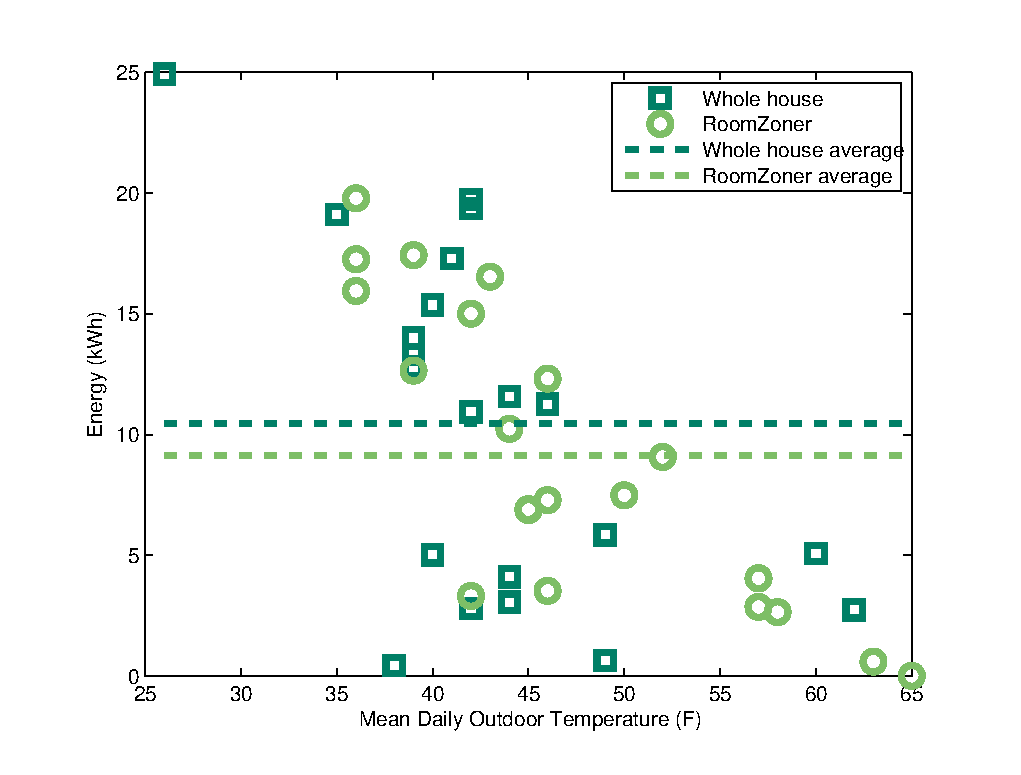
\includegraphics[width=0.6\columnwidth]{fig/cs2scatter.eps}
  \caption[Effect of outdoor temperature on energy usage for RoomZoner]{The
  dotted lines indicate the average energy used over the experimental period.}
  \label{fig:cs2energy}
\end{figure}

Figure~\ref{fig:cs2energy} shows the actual energy consumption for each day as a
scatter plot, with the average temperature of for that day on the x-axis, the
energy consumed on the y-axis, and the control algorithm shown as the color of
the scatter point. 

\subsection{Macroprogramming Discussion}
Extending the Python implementation of day/night zoning to implement RoomZoner
required the introduction of a number of functions to assess occupancy and
dynamically change zones based on room occupancy and temperature changes. This
increased the code size from about 500 lines of code to over 1000 lines of
code. Extending the MacroLab implementation of day/night zoning to RoomZoner saw
a similar doubling in code size from about 200 lines of code to about 500 lines
of code.

Unlike case study 1, the RoomZoner macroprogram cannot be optimized using
in-network data processing or data fusion. This is because the zones dynamically
vary and therefore temperature and motion information from all the rooms are
required to make control decisions. In a large, multi-hop network in-network
data aggregation could be used to aggregate the sensor readings within each room
in order to calculate an average room temperature which is passed up to the base
station, but this optimization doesn't provide as much savings in terms of
messages passed as afforded in the day/night zoning scenario. Thus, due to the
need for more data as the application complexity increases, the flexibility
afforded to MacroLab to perform implementation optimizations
decreases. Table~\ref{table:macrolabOptimizations} summarizes the applicability
of MacroLab optimizations for Dual-Zone and RoomZoner.

\begin{table}[!htb]
  {
  \begin{tabular}{|l|l|l|} \hline
    Optimization & Dual-Zone & RoomZoner\\ \hline\hline
    In-network data processing & Yes & No \\
    In-network aggregation & Yes & Yes \\ \hline
    Data fusion & Yes & No \\ \hline
  \end{tabular}}
  \caption[MacroLab optimizations for case studies]{As the application
  complexity increases the freedom for MacroLab optimizations decreses.}
  \label{table:macrolabOptimizations}
\end{table}

While the benefit of macroprogramming abstractions in terms of implementation
optimization decreases as the application complexity increases, they are still
valuable in implementing CPS applications. Their main value they provide is by
decreasing the burden on the application developer by maximizing code
re-usability and providing a uniform abstraction for data and hardware
accesses. In the case of MacroLab all data within the network is presented as
vectors and all hardware actuations are enabled by function calls. If the
sensors or actuators being used have been previously used for an application
developed using MacroLab, hardware drivers that provide the actuation function
and present the sensor data as vector will be available. If the application is
using a new set of hardware, the drivers would have to be written the first time
after which all future applications could be written assuming the availability
of vectors with sensor data and function to perform actuation. 

\section{Conclusions}
Case study 2 demonstrated the limitation of macroprogramming abstractions, in
terms of code optimization, as application complexity increases. While the
amount of optimizations is limited, the simple high-level programming
abstraction provided by macroprogramming languages makes developing complex CPS
applications easier. Macroprogramming abstractions allow application developers
to focus on describing the application logic as they envision it without being
burdened with collecting the data from the sensors or being concerned with the
passing of messages within the network. Thus, useful CPS applications such as
RoomZoner can easily be developed.

RoomZoner enabled simple COTS sensors and actuators to be used to retrofit a
centralized HVAC system and dynamically change zones based on occupancy. Such
dynamically altering zones resulted in a 14\% energy savings as compared to the
whole house being conditioned as a single zone. RoomZoner is the first system to
enable a centralized HVAC system to be zoned in response to room
occupancy. Incorporating prediction, as described in the next chapter, could
result in even greater energy savings for such a system.


% - Independent vars -> parameters and num sensors
% - Metrics -> FN, short cycle, energy waste
% - Comparison -> - reactive
%                 - uniform
%                 - whole house occupancy
